\documentclass{llncs}
\usepackage{tikz}
\usepackage{amsmath}
\usepackage{amssymb}
% \usepackage{amsthm}	
\usepackage{graphicx}
\usepackage{subcaption}
\usepackage{listings}
\usepackage{float}
\usepackage{minted}
\usepackage{multicol}
\usepackage{ebproof}
\usepackage{array}
\usepackage{xcolor}
\usepackage{stmaryrd}
\usepackage{adjustbox}
\usepackage{wrapfig}
\usepackage{enumitem}
\usepackage{tabularx}
\usepackage{lineno}
\usepackage{mathtools}
\usepackage[hidelinks]{hyperref}
\usepackage{hhline}

\usetikzlibrary{arrows,positioning,shapes}

\allowdisplaybreaks

\usepackage[
style=alphabetic,
sorting=ynt
]{biblatex}

\definecolor{purplell}{HTML}{f72585}
\definecolor{purplel}{HTML}{b5179e}
\definecolor{bluel}{HTML}{4895ef}
\definecolor{bluell}{HTML}{4361ee}
\definecolor{blued}{HTML}{3f37c9}
\definecolor{greend}{HTML}{52b69a}
\definecolor{redl}{HTML}{e63946}
\definecolor{orangel}{HTML}{fb8500}

\lstdefinestyle{deno}{
    language=C,
    captionpos=b,
    numbers=left,
    frame=tb,
    breaklines=true,
    xleftmargin=3em,
    keywordstyle=\color{blue},
    commentstyle=\color{orangel},
    basicstyle=\ttfamily\scriptsize,
    morekeywords={newResource, copy, mut, fn, ref, decl, transfer, borrow, mborrow, call, own, read},
    literate={->}{$\rightarrow$}{2}
}

\lstdefinestyle{deno2}{
    language=C,
    captionpos=b,
    breaklines=true,
    keywordstyle=\color{blue},
    commentstyle=\color{orangel},
    basicstyle=\ttfamily\scriptsize,
    morekeywords={newResource, copy, mut, fn, ref, decl, transfer, borrow, mborrow, call, own, read},
    literate={->}{$\rightarrow$}{2}
}


\lstdefinestyle{osl}{
    language=C,
    captionpos=b,
    numbers=none,
    frame=tb,
    xleftmargin=3em,
    keywordstyle=\color{blue}\upshape,
    basicstyle=\ttfamily\scriptsize,
    morekeywords={newResource, fn, ref, decl, transfer, borrow, mborrow, call, own, read, free, deallocate, unsafe, !, @},
    keywordstyle = [3]{\color{purplel}},
    morekeywords=[3]{copyable,mutable},
    escapeinside={(*}{*)},
    breaklines=true,
    literate={->}{{$\rightarrow$}}1 
    {/\\}{{$\cap$}}1
    {\\/}{{$\cup$}}1
    {'}{{$\'$}}1
}

\lstdefinestyle{clang}{
    language=C,
    captionpos=b,
    numbers=none,
    frame=tb,
    xleftmargin=3em,
    escapeinside={(*}{*)},
    breaklines=true,
    tabsize=2,
    numbers=left,
    basicstyle=\ttfamily\scriptsize,
    keywordstyle=\color{blue}\upshape,
    stringstyle=\color{greend}\ttfamily,
    literate={->}{$\rightarrow$}{2}
}



\newcommand*{\Comment}[1]{\hfill\makebox[5.0cm][l]{#1}}%

\newcommand{\den}[2][]{\llbracket \text{#2} \rrbracket^{#1}}

\newcommand{\autour}[1]{\tikz[baseline]{%
\node[rectangle,rounded corners=0.5mm,text=white,fill=blued!65,inner sep=2pt,anchor=base] (A) {\scriptsize{}#1};}}

% From https://math.berkeley.edu/~gbergman/misc/hacks/langl_rangl.pdf
\newcommand{\langl}{\begin{picture}(4.5,7)
\put(1.1,2.5){\rotatebox{60}{\line(1,0){5.5}}}
\put(1.1,2.5){\rotatebox{300}{\line(1,0){5.5}}}
\end{picture}}
\newcommand{\rangl}{\begin{picture}(4.5,7)
\put(.9,2.5){\rotatebox{120}{\line(1,0){5.5}}}
\put(.9,2.5){\rotatebox{240}{\line(1,0){5.5}}}
\end{picture}}

\newcommand{\lang}{\begin{picture}(5,7)
\put(1.1,2.5){\rotatebox{45}{\line(1,0){6.0}}}
\put(1.1,2.5){\rotatebox{315}{\line(1,0){6.0}}}
\end{picture}}
\newcommand{\rang}{\begin{picture}(5,7)
\put(.1,2.5){\rotatebox{135}{\line(1,0){6.0}}}
\put(.1,2.5){\rotatebox{225}{\line(1,0){6.0}}}
\end{picture}}

\newcommand{\cfg}[1]{\lang #1\rang}

\newcommand{\var}[1]{ \textcolor{purplel}{\textbf{#1}}}
\newcommand{\term}[1]{ \textcolor{blued}{\textbf{#1}}}
\newcommand{\modif}[1]{\textcolor{purplel}{\textbf{#1}}}
\newcommand{\modiff}[1]{\textcolor{bluell}{\textbf{#1}}}
\newcommand{\tagg}[1]{\textcolor{greend}{\textbf{#1}}}
\newcommand{\tagr}[1]{\textcolor{redl}{\textbf{#1}}}
\newcommand{\tago}[1]{\textcolor{orangel}{\textbf{#1}}}

\newcommand{\confosl}{\mathbb{C}}


\newcommand{\letin}[1]{ \textcolor{bluel}{ \textbf{let } } #1 \textcolor{bluel}{ \textbf{ in } } }

% Didactic Semantic =================
\newcommand{\confosld}{(\env,\store)}
\newcommand{\nat}{\mathbb{N}}
\newcommand{\osld}{OSL$_{\mathcal{D}}$}

\def\refrule#1{\hyperref[#1]{\autour{#1}}}

% Operational Semantic =================
\newcommand{\oslt}{OSL$_{\Tau}$}
\newcommand{\osltc}{OSL$_{\Tau C}$}
\newcommand{\oslos}{OSL$_{\mathcal{OS}}$}


\definecolor{purpleTag}{HTML}{8837c9}
\definecolor{blueTag}{HTML}{3778c9}

\newcommand{\tagp}[1]{\textcolor{purpleTag}{\textbf{#1}}}
\newcommand{\tagb}[1]{\textcolor{blueTag}{\textbf{#1}}}
\newcommand{\tagy}[1]{\textcolor{yellowTag}{\textbf{#1}}}
\newcommand{\tagpl}[1]{\textcolor{purplel}{\textbf{#1}}}


\newcommand{\config}{\mathbb{C}}
\newcommand{\env}{\mathcal{E}}
\newcommand{\store}{\mathcal{S}}
\newcommand{\writes}{\mathcal{W}}
\newcommand{\unsafe}{\mathcal{U}}
\newcommand{\envfun}{\mathcal{F}}
\newcommand{\confoslunfold}{(\env,\store,\writes, \unsafe, \envfun)}
\newcommand{\confoslunfoldp}{(\env',\store',\writes', \unsafe', \envfun')}
\newcommand{\confoslunfoldpp}{(\env'',\store'',\writes'', \unsafe'', \envfun'')}


\newcommand{\Tau}{\mathcal{T}}

\captionsetup[sub]{font={bf,small}, name={}, skip=1pt, singlelinecheck=false, labelformat=empty}


% Transpiler =================

\newcommand{\map}{\Gamma}
\newcommand{\out}{\mathcal{O}}
\newcommand{\props}[1]{\pi_{props}(#1)}
\newcommand{\evals}{\xRightarrow[]{\mathcal{S}}}
\newcommand{\evale}{\xRightarrow[]{\mathcal{E}}}

\newcommand{\append}{
  \mathbin{{+}\mspace{-8mu}{+}}%
}


\addbibresource{biblio.bib}

\begin{document}

\title{\textbf{OSL}: A Formalized Ownership Language for Checking Memory Safety}
\author{Anonymous}
%
% \authorrunning{S. Kan et al.}
\titlerunning{OSL: A language for Memory Safety Checking}

% \institute{SCSE,
% 	Nanyang Technological University, Singapore
% 	\email{\{name\}@ntu.edu.sg}
% }

\maketitle

\begin{abstract}
	Ensuring memory safety is an essential issue in software security. Numerous memory safety vulnerabilities are correlated to memory access patterns.
	The ownership system is an efficient and effective mechanism for detecting unsafe memory risks implemented in many languages, such as Rust.
	In this paper,  we propose the framework OSL, which includes an intermediate language called \oslos~to capture the features of the ownership system, and a translator \oslt~to infer ownership properties in C programs by static analysis.
    The C programs translated by \oslt~can be executed  in \oslos~to detect  memory usage vulnerability.
	The ownership semantics is implemented in a formal modeling tool $\mathbb{K}$-Framework, which produces a language-independent formal ownership checker.
	\keywords{Ownership types \and memory aliasing \and static analysis \and C programming language \and $\mathbb{K}$-framework.}
\end{abstract}






\section{Introduction}

Memory aliasing is one of the major challenges that must be addressed when using declarative or imperative language. The term aliasing refers to a situation in which a resource can be accessed through different symbolic names in the program. When aliases access that resource in different ways—such as both reads and writes, there are consequences for the order in which these mixed accesses can happen. In many instances, aliasing is harmless: it is common, safe, and generally efficient to use two aliases to read and even to write to the same resources. But in some cases, using aliasing symbols for mixed accesses is less benign and can adversely affect the correctness of the program by leading to common memory problems such as \textit{data-race},  \textit{double-free} and  \textit{use-after-free}.

To address aliasing pitfalls, Clarke, Potter and Noble have proposed a new design principle called\textit{ Ownership types for flexible alias protection} \cite{10.1145/286942.286947}, which has been continued to be studied \cite{10.1007/978-3-642-36946-9_3}. This technique is a  conceptual model of inter-object relationships. Rather than banning aliasing altogether, the key idea was to limit the visibility of changes to objects via aliases. This was done either by limiting where an alias could propagate or by limiting the changes that could be observed through an alias. Modern languages like Rust \cite{matsakis2014rust}, Cyclone \cite{270632}  and Pony \cite{van2020strengthening} took up this idea, improved it, and can carry out memory safety checking at compile time, while avoiding garbage collection for Rust.
However, these works view the ownership system as a type system \cite{weiss2021oxide}, and their implementation is language-dependent, which makes it hard to reuse it for other languages.
Several solutions have been proposed to add ownership type to languages that do not support this facet \cite{10.1016/j.scico.2006.03.001, 10.1145/3453483.3454036}. These solutions can be classified into two groups: the first one asks the user to annotate the code, the second try to infer Ownership by performing static analysis. Ownership type systems could require considerable annotation overhead, which is a significant burden for users. In the second case,
the resulting effectiveness of the static analysis method depends on the targeted language expressiveness. In our view, helping users transition from unannotated programs to code that uses an Ownership type system is crucial to facilitate the adoption of ownership type systems.\\

In this paper, we propose the Framework: {\em Ownership System Language} (OSL), composed of \oslos~ an independent intermediate language, formalized by an operational semantics instead of a type system; and a translator \oslt, a static analysis tool to infer ownership properties in C programs. The operational semantics characterizes the ownership checking inspired by Rust. Moreover, by having a language-independent, it becomes possible to check ownership properties of programs written in a non-native ownership type like C, Javascript, or Golang. We decided to develop first \oslt~given that numerous of memory safety vulnerabilities are correlated to memory access patterns \cite{CVE-mem-access}.

The semantics of \oslos~has been implemented with $\mathbb{K}$-Framework \cite{rosu-serbanuta-2010-jlap, lucanu-rosu-serbanuta-2012-wrla}, a rewriting logic based formal modeling tool. 
$\mathbb{K}$ has been successfully used to model the semantics of Java \cite{bogdanas-rosu-2015-popl} and C \cite{hathhorn-ellison-rosu-2015-pldi}.
The output of $\mathbb{K}$ is an executable semantics of \oslos, called \textit{K-OSL}. 
Translated C programs by \oslt~ can be executed in \textit{K-OSL} to detect memory usage bugs.
The ownership checking of \oslos~shows that the OSL framework is capable of detecting unsafe memory risks in C programs and being extendable to other declarative programming languages.\newline

\subsubsection{Contributions and Outline.} Our contributions are as follows:
\begin{itemize}
	\item We develop the intermediate language \oslos, which guarantees the properties of an Ownership System.
	An operational semantics is defined for \oslos, characterizing ownership checking.
	\item The  operational semantics of \oslos~is implemented in K-framework, which produces an executable formal semantics.
	The executable can be viewed as an independent formal ownership checker.
    \item We develop a translation tool of C to OSL program called \oslt, in order to check the memory safety guarantee by the Ownership system of \oslos. 
    \item We guarantee that programs validated by OSL are free of dangling pointers, data races, and double free bugs.
\end{itemize} 

The rest of the paper is structured as follows: In \autoref{sec:ownership}, we define our Ownership System principles.
 In \autoref{sec:osl-syntaxandsemantics}, we will first use examples to present how \oslos~prevent memory safety with
 his semantic, followed by an explanation on how \oslt~translate C programs into \oslos~program.
 In \autoref{sec:properties}, we specify the soundness of \oslos w.r.t. dangling pointers, double free, and data races.
 In \autoref{sec:imp-eval}, we describe how we evaluate our semantics and its current limitations.
 We discuss related work in \autoref{sec:relatedwork} and conclude in \autoref{sec:conclusion}.


\section{Ownership System and Memory Safety}
\label{sec:ownership}

\subsection{Illustration of core concepts}
In this section, we introduce our ownership system and how that prevents memory risks: dangling pointers, data races, use-after-free and double free. 
We begin with a synopsis of our semantic, in which we only introduce the main concept with the aid of a simplified didactic semantic of OSL.
The complete operational semantics will be covered in the \autoref{sec:osl-syntaxandsemantics}.\\

OSL works by restricting resource graphs underlying the run-time heap.
That ensures \textit{topological restrictions} on the alias structure of the resource graph.
The core concept of OSL is resource \textbf{owner}, namely each resource in OSL has a variable that’s called its \textbf{owner}.
There exists only one \textbf{owner} at a time for a resource. When the \textbf{owner} goes out of \textbf{scope}, the value will be \textbf{free} in memory.\\

\begin{wrapfigure}{l}{0.5\linewidth}
\centering
\begin{lstlisting}[style=deno]
{ // begin of the scope
    decl x;
    transfer newResource() y;
    decl y; 
    transfer x y;
    { // begin of sub-scope
        decl z;
        z borrow y;                         
        read(z);                            
    } // end of sub-scope
    decl m;                             
    m mborrow y;                        
    transfer newResource() m;  
} // this scope is now over
\end{lstlisting}
\caption{OSL Example}
\label{fig:Didactic-OSL-example}
\end{wrapfigure}

The example \autoref{fig:Didactic-OSL-example} will guide us with the simplified didactic semantics of OSL and the introduction of the main concepts in \autoref{ssec:Formalisation of core concepts}. In this program, a first \textbf{owner} \var{x} is declared (using \term{decl}) at line 2, and we assigned a new resource by using \term{newResource} and \term{transfer} right after.
This means that \var{x} exclusively \textbf{owns} this resource, so he can read, write and deallocate it. There can only be one owner at a time for this resource. Hence, when we \term{transfer} the ownership at line 5, \var{y} becomes the new owner of the resource, and \var{x} stops owning the value. This is called the \textit{move semantics}. Any usage of \var{x} becomes invalid after this. As an aside, the move semantics is powerful in preventing the double free error because each value has a single owner, and only the owner can free the value.\\

Sometimes, multiple variables need to access the same value, but the move semantics requires the program to pass the value between these variables. This could become unergonomic, especially when crossing function boundaries. To improve the usability, we allow a variable to borrow a resource without taking ownership. At the lines 5 and 8, we declare a variable \var{z} that \term{borrow} immutably \var{y}, respectively the variable \var{m} borrow mutable (using \term{mborrow}) \var{y}.
When z borrows the value of \var{y}, \var{y} still owns the resource. A variable can borrow a value for reading only or for both reading and writing. The former is an immutable reference, and the latter is a mutable reference. The mutable reference \var{m} allows mutating the resource owned by \var{y} through \var{m}. This is what happens at line 13, where we \term{transfer} a new resource to \var{y} through \var{m}. We will see in \autoref{sec:osl-syntaxandsemantics} that resources can be defined as immutable, so a variable may mutably borrow a variable only if it is defined as mutable.\\

When \var{z} goes out of the sub-scope at line 9, the borrow ends, and since \var{z} does not own the resource, the resource isn't destroyed. The \textbf{lifetime} of a variable is from where it is bound to where it goes out of scope. Each reference has a lifetime that must be contained in the lifetime of the borrowed content. In our case, the reference \var{z} has a lifetime that begins at lines 7 and ends at 9. Respectively, the reference \var{m} lives between 11-13 and \var{y} lives between 4-13. We can assert that given Lifetime(y) = [4-13], we have $Lifetime(z) \subset Lifetime(y)$, $Lifetime(m) \subset Lifetime(y)$ and $Lifetime(z)  \cap Lifetime(m) = \emptyset$.


\subsection{Formalization of  core concepts}
\label{ssec:Formalisation of core concepts}

To formalize the ownership system concepts, we first introduce a didactic version of OSL that we will name \osld, which is a fragment of the complete OSL framework cover in \autoref{sec:osl-syntaxandsemantics}. It will help us to introduce more clearly the formalization of the core concepts.
\osld is composed of only a few operators, which are presented in \autoref{lst:didactic-syntax}. Our previous example \autoref{fig:Didactic-OSL-example} covers mainly this abstract syntax. We add just the statement \term{read} that allows us to read the value of an owner or a reference. For the sake of simplicity, \term{read} will check the validity of the parameter and not return a value.

\begin{lstlisting}[caption=\osld~abstract syntax,style=deno,label=lst:didactic-syntax]
Exp ::= newResource() | Id
Stmt ::= Stmt ; Stmt | Id borrow Id | Id mborrow Id
     | decl Id | transfer Exp Id | read Id | { Stmt }
\end{lstlisting}

\begin{definition}[State representation]
A \textbf{state} of \osld~is defined as a triple $\cfg{\confosl , P, t }$, where the \textbf{environment} $\confosl$ is a tuple $\confosld$ with:
\begin{itemize}[noitemsep]
    \item[] $\env:Id\mapsto Loc$, a map from variable to location representing an environment for variables .
    \item[] $\store:Loc\mapsto Value$, a map from location to value storing values for locations.
\end{itemize}
The location $Loc$ is defined by a natural number. $P$ is the program to be executed under the configuration $\confosl$ at the time instant: $t$.
A state is initialized as $\cfg{(\emptyset,\emptyset),P, 0}$ where the environment is are empty and the timer starts at 0.
\end{definition} 

\subsubsection{Domain value.}

The domain below represents all possible $Value$ that a location can map to in $\store$.
We use the notation $\bot$ as the least element to describe an uninitialized location.
The notation $\#rs()$ denotes a resource. The notations $\text{mutRef}(\mathbb{N}, \mathbb{N}, Loc)$,
$\text{immRef}(\mathbb{N}, \mathbb{N}, Loc)$ represent a mutable and an immutable reference, respectively,
where the two natural numbers represent a lifetime span.

\begin{equation*}
    Value = \Big\{~\#rs(),~ \bot,~ \text{mutRef($\mathbb{N}, \mathbb{N}$, Loc)},~ \text{immRef($\mathbb{N}, \mathbb{N}$, Loc)}~\Big\}
    \label{eqn:value-d}
\end{equation*}

\subsubsection{Presentation of core concepts.} We use the notation $\oplus$ to represent the update of a state.
For example, $\store' = \store \oplus [L \mapsto V]$ will update the state $\store$ with the assignment $L = V$  and accordingly we have $\store'[L] = V$.
\begin{figure}
    % Declaration =========================
    \begin{subfigure}{0.5\textwidth}
        \subcaption{\autour{Decl}}
        \centering
        \begin{prooftree}
            \hypo{\begin{matrix}
              \textit{l = new\_loc} \\
              \env' = \env \oplus [x \mapsto l]
            \end{matrix}}
            \hypo{
              \store' = \store \oplus [l \mapsto \bot]
            }
            \infer2[]{ \cfg{ \confosld, \term{decl } x;, t} \Rightarrow  \cfg{(\env', \store'), \emptyset, t + 1}}
        \end{prooftree}
    \end{subfigure}
    % NewResource =========================
    \begin{subfigure}{0.4\textwidth}
        \centering
        \subcaption{\autour{ResExp}}
        \begin{prooftree}
            \infer0[]{ \cfg{\confosl, \term{newResource(), t}} \Rightarrow \cfg{\confosl, \term{\#rs()}, t} }
        \end{prooftree}
    \end{subfigure}
    \caption{Owner rules of \osld}
    \label{fig:dec-rule-osld}
\end{figure}

\begin{definition}[Owner]
For all $ x \mapsto l \in \env \text{ with } l \mapsto \#rs() \in \store,$ x is called the \textbf{owner} of the resource.
\end{definition}

\begin{definition}[Unique Owner]
\label{def:unique-owner}
For all $x \mapsto l_1 \text{ and } y \mapsto l_2 \in \store, \textbf{ if } \text{ we have }\\  l_1 \mapsto \#rs() ~\land~ l_2 \mapsto \#rs() \text{ with } l_1 = l_2  \text{, then that implies } x = y$.
\end{definition}

\begin{figure}
    \begin{subfigure}{\textwidth}
    \vspace*{-0.5cm}
    \centering
        \begin{prooftree}
            \hypo{
                \begin{matrix}
                    (x \mapsto l_1~, y \mapsto l_2) \in \env \\
                    l_1 \mapsto \#rs() \in \store
                \end{matrix}
            }
            \hypo{
              \store' = \store \oplus [l_1 \mapsto mutRef(\tagp{t, t}, l_2)]
            } x
            \infer2[\autour{Borrow}]{ \cfg{ \confosl, x \term{ mborrow } y;, \tagp{t}} \Rightarrow  \cfg{(\env , \store'), \emptyset, t + 1}}
        \end{prooftree}
     \vspace*{0.3cm}
     \label{Borrow}
    \end{subfigure}
    \begin{subfigure}{\textwidth}
        \centering
        \begin{prooftree}
              \hypo{
                \begin{matrix}
                    (x \mapsto l_1,~y \mapsto l_2) \in \env \\
                    l_2 \mapsto \#rs() \in \store
                \end{matrix}
            }
            \hypo{
              \store' = \store \oplus [l_1 \mapsto immRef(\tagp{t, t}, l_2)]
            }
            \infer2[\autour{MBorrow}]{ \cfg{ \confosl, x \term{ borrow } y;, \tagp{t}} \Rightarrow  \cfg{(\env , \store'), \emptyset, t + 1}}
        \end{prooftree}
        \label{MBorrow}
    \end{subfigure}
    \caption{Borrowing rules of \osld}
   
\end{figure}

\begin{definition}[Multiples reference restriction]
At any given time, you can have either one mutable reference active or any number of immutable references active. 
\label{def:mult-ref}
\end{definition}

The lifetime span [\tagp{$t_1, t_2$}] in mutRef(\tagp{$t_1, t_2$}, l) and immRef(\tagp{$t_1, t_2$}, l) defines when the reference is active. Thus the reference has the current timer value as lower and greather bound  as lifetime span in  in \refrule{MBorrow} and respectively \refrule{Borrow}. The semantics of the operators \term{mborrow} and \term{borrow} in \refrule{MBorrow} and respectively \refrule{Borrow} do not restrict us in creating references for an owner. But we will see in the following rule \refrule{ReadRef}, we can only \term{read} through a reference if there are not other active mutable references to the same owner to be in accord with \autoref{def:mult-ref}.

\begin{definition}[Create reference]
A reference to a resource can only be created through the owner.
\label{def:create-ref}
\end{definition}

\begin{definition}[Immutable reference]
When an immutable reference is active, no writing is allowed to its owner.
\label{def:imm-ref}
\end{definition}

\begin{definition}[Active reference freeze owner]
When a resource has a mutable reference, the resource owner is temporally invalid while the reference is within its lifetime.
\label{def:freeze-owner}
\end{definition}

This property allows OSL to prevent a data-race by refusing a potential attempt to access a resource through the owner and a mutable reference to it with intersecting lifetimes.  
The simple model of \osld~does not allow for covering the \autoref{def:freeze-owner}. But we will present how OSL captures this property in \autoref{sec:osl-syntaxandsemantics}.

\noindent We use the notation $\term{anyRef}(t_b, t_e, L)$ to denote any mutable or immutable reference in $\store$.

\begin{figure}[H]
    \begin{subfigure}{\textwidth}
        \centering
        \begin{prooftree}
         \hypo{
            \begin{matrix}
            x \in Id \\
            x \mapsto l_x \in \env  \land l_x \mapsto v \in \store  \\
             \nexists l \mapsto \term{immRef}(t_b, t_e, l_y) \in \store \land t_e \geq t
            \end{matrix}
         }
        \hypo{
            \begin{matrix}
            y \mapsto l_y \in \env \\
            S'=S \oplus [l_y \mapsto  v,  l_x \mapsto \bot ]
            \end{matrix}
         }
        \infer2[\autour{Tmove}]{ \cfg{ \confosld, \term{ transfer } x~y; , t } \Rightarrow  \cfg{ (\env, \store'), \emptyset, t + 1 } }
        \end{prooftree}
        \vspace*{2em}
        \label{Tmove}
    \end{subfigure}
    \begin{subfigure}{\textwidth}
        \centering
        \subcaption{\autour{TMborrow}}
        \begin{prooftree}
         \hypo{
            \begin{matrix}
                x \in Id \\
                x \mapsto l_x \in \env  \land l_x \mapsto \tagp{v} \in \store  \\
                \nexists l \mapsto \term{anyRef}(t_b, t_e,  \tagb{$l_c$}) \in \store \land t_e \geq t
            \end{matrix}
         }
        \hypo{
            \begin{matrix}
            y \mapsto l_y \in \env \\
            l_y \mapsto mutRef(tb_y, te_y, \tagb{$l_c$}) \in \store \\
            S'=S \oplus [\tagb{$l_c$} \mapsto  \tagp{v}, l_y \mapsto mutRef(tb_y, t, \tagb{$l_c$}) ]
            \end{matrix}
         }
        \infer2[]{ \cfg{ \confosld, \term{ transfer } x\ y; , t } \Rightarrow  \cfg{ (\env, \store'), \emptyset, t + 1 } }
        \end{prooftree}
        \label{TMborrow}
        \vspace*{2em}
    \end{subfigure}
    \begin{subfigure}{\textwidth}
        \centering
        % TRANFER RESOURCE =========================
        \begin{prooftree}
         \hypo{
           \begin{matrix}
                \cfg{ \confosld, e, t } \Rightarrow  \cfg{ \confosld , \#rs(), t } \\
                x \mapsto l \in \env
            \end{matrix}
         }
        \hypo{
            \store' = \store \oplus (l \mapsto \#rs(r))
         }
        \infer2[\autour{Tres}]{ \cfg{ \confosld, \term{ transfer } e~x;, t } \Rightarrow  \cfg{ (\env, \store'), \emptyset, t+1 } }
        \end{prooftree}
        \label{Tres}
    \end{subfigure}
    \caption{Transfer rules of \osld}
    \label{fig:transfer-rule-osld}
\end{figure}

\begin{definition}[Transfer owner]
\label{def:transfer}
The ownership of a resource can be transferred among owners. 
\end{definition}

We illustrate this in rule \refrule{Tmove}, where the \textbf{owner} \term{x} of \term{v} is transferred to \term{y}. Then \term{y} maps to v and \term{x} maps to $\bot$.
This concept can also be found in the literature under the name: \textit{semantic move}. 

\begin{proposition}{}
Since references do not own the value, they cannot move it.
\end{proposition}

\begin{figure}[H]
    % Read Owner =========================
    \begin{subfigure}{0.5\textwidth}
        \subcaption{\autour{ReadOwner}}
            \begin{prooftree}
             \hypo{
                x \mapsto l \in \env
             }
            \hypo{
                l \mapsto \#rs() \in \store    
             }
            \infer2[]{ \cfg{ \confosld, \term{ read}(x);, t } \Rightarrow  \cfg{ \confosld, \emptyset, t+1 } }
        \end{prooftree}
    \label{ReadOwner}
    \end{subfigure}
    \begin{subfigure}{0.5\textwidth}
        \subcaption{\autour{ReadRef}}
        \begin{prooftree}
            \hypo{
            \begin{matrix}
                l \mapsto \#ref(\tagb{$t_b, t_e$}, l) \in \store \\
                \nexists l' \mapsto mutRef(\tagp{$t_b', t_e'$}, l) \in \store, \\
                \text{with } \tagp{$t_b'$} \leq \tagb{$t_b < t_e$} \leq \tagp{$t_e'$} \\
                \store' = \store \oplus [ l \mapsto \#ref(t_b, t, l) ]
            \end{matrix}
            }
            \hypo{
            \begin{matrix}
                x \mapsto l \in \env
            \end{matrix}
            }
            
            \infer2[]{ \cfg{ \confosld, \term{ read}(x);, t } \Rightarrow  \cfg{ (\env, \store'), \emptyset, t+1 } }
        \end{prooftree}
        \label{ReadRef}
    \end{subfigure}
    \caption{Read rules of \osld}
\end{figure}

As mentioned in an observation of \autoref{def:mult-ref}, the predicate: $\\ \nexists l' \mapsto mutRef(t_b', t_e', l) \in \store ~with~ \tagp{$t_b'$} \leq \tagb{$t_b < t_e$} \leq \tagp{$t_e'$}  $ in the rule \refrule{ReadRef} allow us to respect the definition.


\begin{figure}[H]
    \begin{subfigure}{0.6\textwidth}
    % Seq =========================
        \centering
        \subcaption{\autour{Seq}}
        \begin{prooftree}
         \hypo{
            \cfg{ \confosl, s1, t } \Rightarrow  \cfg{\confosl' , \emptyset, t_1 }
         }
        \hypo{
            \cfg{ \confosl', s2, t_2 } \Rightarrow  \cfg{ \confosl'', \emptyset, t_2 }
        }
        \infer2[]{ \cfg{ \confosl, s1 ; s2, t } \Rightarrow  \cfg{ \confosl'', \emptyset, t_2 } }
        \end{prooftree}
        \label{Seq}
    \end{subfigure}
    \quad
    \begin{subfigure}{0.3\textwidth}
        \centering
      \subcaption{\autour{Block}}
        \begin{prooftree}
         \hypo{
            \cfg{ \confosl, s, t } \Rightarrow  \cfg{\confosl' , \emptyset, \tagb{t'} }
         }
        \infer1[]{ \cfg{\tagp{$\confosl$}, \textbf{\{} s \textbf{\}} , t } \Rightarrow  \cfg{\tagp{$\confosl$}, \emptyset, \tagb{t'} } }
        \end{prooftree}  
        \label{Block}
    \end{subfigure}
    \caption{Sequence and block  rules of \osld}
\end{figure}

\begin{definition}[Free owner automatically]
\label{def:free-owner}
When an \textbf{owner} goes out of scope, its resource will be dropped. Automatically, the resources and their respective owners allocated inside the scope are cleaned up at the end of a block.
\end{definition}

To illustrate the \autoref{def:free-owner}, we can observe in the rule \refrule{Block} that after we evaluate the statements inside the block, we restore the previous configuration \tagp{$\confosl$}.
So all the owners and references declared inside will be dropped. 

\begin{definition}[Deallocation restriction]
Only the resource owner has the authority to free the resource manually.
\end{definition}

 We keep this advanced concept for \autoref{sec:osl-syntaxandsemantics} where we introduce the \term{free} operator.

\begin{proposition}{}
The lifetime of a reference is always shorter than its owner's lifetime. In other words, the references do not escape the scope of their referent.
The scope of a reference must be contained in the owner's scope of the value. Otherwise, the reference may refer to a freed value, causing a use-after-free error.
\end{proposition}


\subsection{Overview of memory safety properties}

In all programming that uses memory, we desire two program properties: \textit{Memory safety} and \textit{Memory containment}.
Memory safety is the property of a program where memory pointers always point to valid memory.
Memory safety is a correctness issue, and an unsafe memory program may crash or produce non-deterministic output depending on the bug.
Memory leaking is a performance issue, and a leaky program may eventually run out of memory is the property of a program where memory does not leak.\\
A common bug related to pointers and memory management is dangling/wild pointers. Sometimes the programmer fails to initialize the pointer with a valid address, then this type of initialized pointer is known as a dangling pointer in C. OSL (even \osld) will prevent us from dandling pointers. Let us unwind this a bit.

\begin{proposition}[Preventing dandling pointers.]
Given any state \cfg{($\env, \store$), P, t}, for all possible derivations of program $P$, it satisfies that given any reference $l \in \store$ with $l \mapsto \term{anyRef}([t_b, t_e], l')$
, there does not exist a state $\cfg{(\env' \store'), P', t'}$ derived from  $\cfg{\confosl, P, t}$, such that  $l \mapsto  \term{anyRef}([t_b, t_e'], l') \in \store'$ hold with  $t' \in [t_b, t_e']$ and $l' \mapsto \bot \in \store'$.
\end{proposition}

\noindent
We will cover in more detail the soundness questions in \autoref{sec:properties}.

\section{Overview of OSL}
\label{sec:osl-syntaxandsemantics}

\lstdefinestyle{mystyle}{
    backgroundcolor=\color{backcolour},   
    commentstyle=\color{codegreen},
    keywordstyle=\color{magenta},
    numberstyle=\tiny\color{codegray},
    stringstyle=\color{codepurple},
    basicstyle=\ttfamily\footnotesize,
    breakatwhitespace=false,         
    breaklines=true,                 
    captionpos=b,                    
    keepspaces=true,                 
    numbers=left,                    
    numbersep=5pt,                  
    showspaces=false,                
    showstringspaces=false,
    showtabs=false,                  
    tabsize=2
}


\begin{wrapfigure}{l}{0.4\linewidth}
\centering
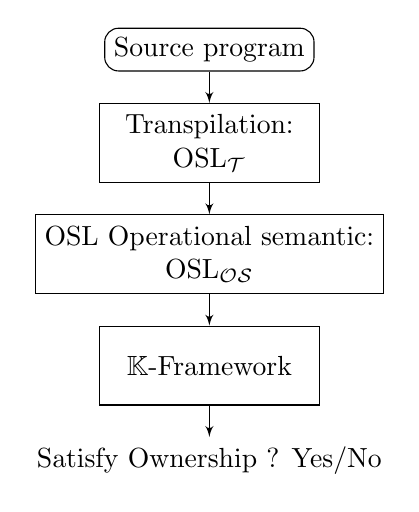
\begin{tikzpicture}[node distance=4mm, >=latex',
             block/.style = {draw, rectangle, minimum height=10mm, minimum width=28mm,align=center},
            rblock/.style = {draw, rectangle, rounded corners=0.5em},
]
\node [rblock]                      (src)     {Source program};
\node [block, below=of src]       (oslt)   {Transpilation:\\OSL$_{\Tau}$};
\node [block, below=of oslt]     (osls)  {OSL Operational semantic:\\OSL$_{\mathcal{OS}}$};
\node [block, below=of osls]     (kf)  {${\mathbb{K}}$-Framework};
\node [below=of kf]     (result)  {Satisfy Ownership ? Yes/No};
%% paths (borowed from Harish Kumar)
\path[draw,->] (src)      edge (oslt)
               (oslt)    edge (osls)
               (osls)    edge (kf)
               (kf)    edge (result)
                ;
\end{tikzpicture}
\caption{An overview of the OSL pipeline}
\label{fig:my_label}
\end{wrapfigure}


We present the OSL semantics and syntax. The OSL analyzer is parametric and may be instantiated for a multitude of declarative and imperative programming languages. The OSL pipeline analysis is divided into two parts. The frontend \oslt, take a C program and translates it into an OSL program. We will present \oslt~in  \autoref{ssec:overview-oslt}. The core \oslos~relies on the rewrite-based executable semantics: ${\mathbb{K}}$-Framework, and encodes our ownership semantics of \autoref{sec:ownership}, and verify the soundness of the program translated by \oslt. The composition of  \oslos~and \oslt~allow us to verify the ownership soundness of many C programs. A new programming language can be supported by extending the translator. \\
In the following sections, we first present the \oslos. How this operational semantic allows us to detect memory bugs, and after will we introduce \oslt. 

\subsection{Overview of \oslos }

\subsubsection{Syntax.}

We built OSL$_{\mathcal{OS}}$ on a simple syntax comprising standard composite commands and parametrized by a set of atomic commands. This allows us to instantiate OSL for several use cases without changing the underlying meta-theory. Our syntax  is given by the \autoref{lst:syntax-osl} below, and includes the didactic syntax \autoref{lst:didactic-syntax} presented in \autoref{ssec:Formalisation of core concepts}; with the exception that \term{read} belongs to expression here. \\ 

\begin{lstlisting}[float=ht,caption=OSL$_{\mathcal{OS}}$ syntax, style=osl,label=lst:syntax-osl]
exp   ::= Id | newResource(props) | (*$\star$*) exp
        | call exp (exps) | read(exp) | & exp | &mut exp
exps ::= exp, ..., exp
prop ::= copyable | mutable
props ::= prop, ..., prop
type ::= own(props) | ref(lifetime, type) | #voidTy
lifeftime ::= (*$'Id$*)
stmt ::= exp ; | decl Id ; | exp borrow exp | exp mborrow exp;
        | transfer exp exp ; | free exp; | @ block, ..., block ;
        | ! block ; | val(exp) ; | stmt stmt | block | unsafe block
block ::= { stmt }
function ::= fn Id < annotations > ( parameters ) (*$\rightarrow$*) type block
annotations ::= lifeftime : annotations  | lifetime
            | annotations \/ annotations | annotations /\ annotations
parameters ::= id: type, ..., id: type
PGM ::= stmt
\end{lstlisting}

Similarly, resources are allocated by \term{newResource}($props$) operator, but a new resource can have properties: $props$. We now only consider the property \tagpl{copyable} and \tagpl{mutable}.
The set of properties is extensible to enable OSL to study a larger class of memory properties in the future.
The \term{transfer}, \term{borrow} and \term{mborrow} statements deal mainly in the same way that the corresponding in \osld.
They only vary on the precondition assertions because of the complete configuration of \oslos~change.  
The property \tagpl{copyable} matters here. When a \tagpl{copyable} resource  is transferred  from $e_1$ to $e_2$, a new resource with the same properties is created and its ownership is transferred to $e_2$.
If a resource is not \tagpl{copyable}, then we proceed to a semantic move.
The expressions \term{\& x} and \term{\&mut x} create a reference for $x$.
The opposite of referencing by using \term{\&}  is dereferencing, which is accomplished with the dereference operator \term{$\star$}.
The symbol \term{@} and \term{!} are respectively the branch and loop operators.
A block of code can be prefixed with the \term{unsafe} keyword to permit unsafe operations like creating multiples mutable alias within a safe block.
\subsubsection{\oslos~Model}

\begin{definition}[A \oslos~configuration]
    A \oslos~\textbf{configuration} is defined as a Set of \textbf{state} triple $\cfg{ (\confosl, P, t), CS }$, where $\confosl$ is called an \textbf{environment} tuple $\confoslunfold$, $P$ is program to be executed under environment $\confosl$ and time counter $t$, and we note $CS$ the tail of the Set. A \textbf{configuration} Set his always initialize as a unit-set with triple $\cfg{ \cfg{(\emptyset,\emptyset,\emptyset, \emptyset, \bot), P, 0}}$, where $P$ is the program and the time counter is set at 0.
\end{definition}


Compared with \osld, we use a set of triple state in \oslos~because it supports conditional statement \term{@}. Therefore, to cover all possible execution paths, \oslos will analyze all of them in different states; more details is provided in \autoref{ssec:flow-control}.  The \textbf{environment} tuple  $\confoslunfold$ is composed by the same $\env$ and $\store$ of \osld~ in \autoref{ssec:Formalisation of core concepts}, but we add : \\

\begin{itemize}
    \item[] $\writes: \{ (L, T)  \mid L \in Loc \land T \in \mathbb{N} \}$, is a set recording the writing for locations together with the 
    time instants at which the writings are carried out. $\term{write}(l,t)\in \writes$ denotes a writing operation on $l$ at the time instant $t$.\\

    \item[] $\unsafe:\mathbb{B}$, is a boolean flag that indicate if we enter in unsafe mode. In this mode, some precondition assertions are no longer required. \\
  
    \item[] $\envfun: Id \mapsto (\text{annotations}, \text{parameters}, \text{type}, \text{block})$, a map from $Id$ to a function definition.   
\end{itemize}

Adding $\writes$ will allow us to satisfy the \autoref{def:freeze-owner} and \autoref{def:imm-ref}. For $\unsafe$, to avoid that \oslos~ reject some program because it does not have enough information to be confident. The user can use \term{unsafe} keyword to tell \oslos: \textit{"Trust me, I know what I’m doing."}. The downside is that bugs such as \textit{null pointer dereferencing} can occur in an incorrect code put inside an \term{unsafe} block. Intuitively the map $\envfun$ stores the definition of the function declared and jumps to them when the keyword \term{call} is used.

\subsubsection{Domain.}

The domain of values stored in $\mathcal{S}$ is defined as follows:

\begin{equation*}
    \begin{aligned}
    Value ::&= \#\textbf{rs}(\tagp{props}) \mid  (\mathbb{N}, \mathbb{N}, \textbf{mutRef}(Loc)) \\
    & \mid (\mathbb{N}, \mathbb{N}, \textbf{immRef}(Loc)) \mid \bot \\
    \end{aligned}
\end{equation*}

Compared to \osld~, here resources can be parametrized to indicate if there are \tagp{mutable} or \tagp{copyable}.

\subsection{\oslos~for Detecting memory usage bugs}
\label{ssec:detecting-mem-bugs}

\oslos~has an operational semantic design to detect misuse memory. Violations include use after free, null pointer dereference, using uninitialized memory and double free.
Memory violations like these can cause programs to crash unexpectedly and be exploited to alter intended behavior. Potential consequences of a memory-related bug include information leakage, arbitrary code execution, and remote code execution. According to the statistical report of MITRE \cite{cwe}, these memory-safety bugs are enumerated among the top dangerous software vulnerabilities.
In this section, we will show how the operational semantic of \oslos~ aims to prevent this error. The complete semantic can be found in Appendix \ref{app:complete-oslos}.

\subsubsection{Use after free.}

\begin{wrapfigure}{R}{0.4\linewidth}
\begin{lstlisting}[style=deno]
decl x;
transfer newResource(mut) x;
decl y;
y borrow x;

free(x);
transfer newResource(mut) y;
* y;
\end{lstlisting}
\caption{use after free}
\label{lst:use-after-free}
\end{wrapfigure}

After freeing a pointer, the buffer pointed by the pointer would be deallocated or recycled. However, the pointer still points to the deallocated memory address. These pointers are named dangling pointers. Dereferencing a dangling pointer causes use-after-free issues. Such bugs are dangerous because the freed memory may have already been reallocated for other
purposes, or it may allow users to control the linked list of free memory blocks maintained by the system and achieve arbitrary write \cite{217626}. In the example \autoref{lst:use-after-free}, \term{y} borrow mutably \term{x} at line 5, and then deallocate the resource owned by \term{x}. Consequently, \term{y} become a dangling pointer, and writing to it or dereferencing causes a use-after-free issue. But the semantic rule \autour{Transfer-mutRef} and \autour{Dereference} prevent this violation. The predicate $ write(\term{wv}(e',E''),t_c)$ will not be validated because we can transfer the resource to \term{y} when the lifetime of \term{y} does not intersect with the owner \term{x}. If we omit the \term{transfer}, the predicate $\cfg{ \confosl', \term{read}(l) } \Rightarrow \cfg{ \confosl'', v }$ in \autour{Dereference} will not be validated because \term{x} it is mapping to $\bot$ after the frees.

\begin{figure}
\begin{subfigure}{\textwidth}
    \subcaption{\autour{TrMutRef}}
    \begin{prooftree}
        \label{TrMutRef}
        \hypo{
            \begin{matrix}
                \cfg{ (\confosl,\term{lv}(\tagp{e1}), t) } \Rightarrow \cfg{ (\confosl',l , t)} \\
                l\mapsto_{lf(\_,\_)} \term{mutRef}(l_1)\in S \\
                \confosl''= \confoslunfoldpp \\
                \nexists l_n\mapsto_{lf(t_b,t_e)}\term{anyRef}(l),t_e\geq t_+
            \end{matrix}
        }
        \hypo{
            \begin{matrix}
                t_+ = t + 1 \\
                \cfg{(\confosl',  \term{lv}(\tagb{e2}), t)} \Rightarrow \cfg{(\confosl'',l', t)} \\
                \store'''=\store'' \oplus (l' \mapsto_{lf(t_+,t_+)} \term{mutRef}(l_1)) \oplus (l \mapsto \bot) \\
                \writes'''= \writes''\cup\{write(\term{wv}(\tagb{e2}, \env''),t_+)\}
            \end{matrix}
        }
        \infer2[]{ \cfg{(\confosl, \term{transfer } \tagp{e1}~\tagb{e2};, t), CS} \Rightarrow \cfg{((\env'',\store''',\writes''', \unsafe, \envfun), \emptyset , t_+) , CS} }
    \end{prooftree}
\label{fig:Transfer-mutRef}

\vspace*{0.5cm}
\end{subfigure}

\begin{subfigure}{\textwidth}
    \centering
    \begin{prooftree}
         \hypo{\cfg{ (\confosl,\term{lv}(*e), t)} \Rightarrow \cfg{(\confosl', \tagp{l}, t)} }
         \hypo{\cfg{ (\confosl',\term{read}(\tagp{l}),t)} \Rightarrow \cfg{(\confosl'',\tagp{v},t)} }
        \infer2[\autour{Dereference}]{ \cfg{ (\confosl, * e, t), CS } \Rightarrow  \cfg{ (\confosl'' , \tagp{v}, t), CS } }
    \end{prooftree}
    \label{fig:deref-rule}
\end{subfigure}
\end{figure}


\subsubsection{Double free.}



\begin{wrapfigure}{r}{0.4\linewidth}
\begin{lstlisting}[style=deno]
decl x;
transfer newResource(mut) x;
free(x);
free(x);
\end{lstlisting}
\caption{Double free}
\label{lst:double-free}
\vspace{-70pt}
\end{wrapfigure}

Freeing a pointer twice causes double free issues. It leaves room for attackers to manipulate the free memory
blocks. Consequently, attackers may overwrite any memory cell of the process leveraging memory allocation system calls.\\\\
In the example \autoref{lst:double-free}, the \term{free} at line 4 will not be validated because \term{x} maps to $\bot$ after the previous \term{free}. So the predicate $\nexists~l \mapsto \bot \in \store$ in \autour{Free} is not valid and \oslos~will return that the program is unsound.

\vspace{0.2cm}
\begin{prooftree}
    \vspace{\baselineskip}
    \hypo{
        \begin{matrix}
            \confosl = \confoslunfold \\
            \cfg{ (\confosl, \term{lv}(x),t) } \Rightarrow \cfg{ (\confosl, l, t) } 
        \end{matrix}
    }
    \hypo{ \tagp{$\store'$} = \store \oplus (l \mapsto \bot ) }
    \hypo{ \nexists~l \mapsto \bot \in \store }
    \infer3[\autour{Free}]{ \cfg{ (\confosl, \term{free}(x), t), CS } \Rightarrow { \cfg{ ((\env, \tagp{$\store'$},\writes, \unsafe, \envfun), \emptyset,t+1), CS } } }
\end{prooftree}


\subsubsection{Uninitialized memory access.}

\begin{wrapfigure}{r}{0.4\linewidth}
    \begin{lstlisting}[style=deno]
    decl x;
    decl y;
    decl z;
    read(x);
    y borrow x;
    z mborrow x;
    read(y);
    read(z);
    \end{lstlisting}
\caption{Uninitialized access}
\label{lst:uninit-mem}
\end{wrapfigure}

It means the memory is used without proper initialization.
Intuitively, it may leak the old content. If the memory contains values of pointer types, falsely accessing or free the pointer would cause invalid memory access. In the rules \autour{Read-Rs}, \autour{Read-immRef} and \autour{Read-mutRef}, all are protected by a predicate from uninitialized memory access. If we try to apply \autour{Read-Rs} at line 2, then the predicate $l \mapsto \#rs(ps) \in S$ will not be satisfy with \term{x}. The variable \term{x} is still mapping to $\bot$, because we did not \term{transfer} a resource. 
Let's analyze another case  when we try to apply \autour{Read-Rs} or \autour{Read-Rs}. The common predicate $\cfg{(\env,\store', \dots),\term{read}(l')} \Rightarrow^+ \cfg{(\env,\store'', \dots),\#rs(\_)}$ where \term{x} is $l'$,  will not be validated. Indeed 
both \term{y} and \term{z} borrow the owner \term{x}, but \term{x} is uninitialized which violate the previous common predicate that requires an initialized owner.

\begin{figure}[H]
    % READ RS ==============
    \begin{subfigure}{\textwidth}
        \centering
        \subcaption{\autour{Read-Rs}}
        \begin{prooftree}
            \hypo{\tagp{l} \mapsto \tagb{\#rs(ps)} \in \store}
            \infer1[]{ \cfg{ (\confoslunfold, \term{read}(\tagp{l}), t), CS} \Rightarrow  \cfg{ (\confoslunfold, \tagb{\#rs(ps)},t), CS }}
        \end{prooftree}
        \label{fig:read-rs}
        \vspace{0.5cm}
    \end{subfigure}
    % READ SHR REF ============
    \begin{subfigure}{\textwidth}
        \centering
        \subcaption{\autour{Read-immRef}}
        \begin{prooftree}
         \hypo{\begin{matrix}
            l \mapsto_{lf(t_b,t_e)} \term{immRef}(l')\in \store \\
            \store' = \store \oplus [l \mapsto_{lf(t_b,t_+)}\term{immRef}(l')] \\
            \cfg{ ((\env, \store', \writes,\unsafe,\envfun), \term{read}(l'), t)} \Rightarrow^+ \cfg{(\confosl'' ,\#rs(\_), t)} \\
            \nexists l_1\mapsto_{lf(t_b',t_e')} \term{mutRef}(l')\in S, l\neq\l_1 \\
         \end{matrix}}
         \hypo{\begin{matrix}
            \neg\term{wl}(l',t_b,t_+,\writes) \\
            \term{lc}(t_b,t_+,t_b',t_e') \\
            t_+= t + 1 \\
         \end{matrix}}
        \infer2[]{ \cfg{ ( \confoslunfold , \term{read}(l), t),CS } \Rightarrow  \cfg{ (\confosl'', l', t_+), CS } }
        \end{prooftree}
    \end{subfigure}
    \begin{subfigure}{\textwidth}
        \centering
        \begin{align*}
            & \textbf{lc}(t_1,t_2,t_3,t_4)\triangleq (t_1< t_3\leq t_2)\lor (t_1\leq t_4\leq t_2) \\
            & \textbf{wl}(l,t,t',W)\triangleq \exists write(l,t'')\in W \land t \leq t'' \leq t'
        \end{align*}        
    \label{fig:read-rs}
    \end{subfigure}

    \label{fig:Read-immRef}
\end{figure}

\subsection{Overview of \oslt}
\label{ssec:overview-oslt}

We next present the operational semantics of \oslt. It automatically translates C programs into the mid-level intermediate representation (MIR) OSL syntax.
Currently, we support the complete  C11  standard version syntax and programs that do not include \textbf{goto} statement. However, we aim to support the translation of any C program.


\subsubsection{\oslt~States.} A \oslt~\textit{state} is a Triple $\cfg{P , \map, \out }$, where $P$ is a list of C tokens,
$\map$ is a map between \textit{Identifier} (variable, function name) to \oslos~\term{Type}, and $\out$ is a Monoid ($O$, $\append$) where $O$ is a \oslos~ program, the associative binary operation $\append$ is the \textit{append} function and the \textit{zero} element $\epsilon$ represent the empty list.
The \textit{triple} $(P, \emptyset, \epsilon)$ is the initial \textit{triple} of \oslt.


\subsubsection{Transpilation of C program.}  The transition between Triple is denoted by $\Rightarrow$. For C expression, the final value is the corresponding translated expression; for C Statement, it is the translated statement with the $\map$ enriched with new variables and functions declared in $P$.

\begin{align*}
&\evale ~::  ( Exp \times Env ) \rightarrow Output \\
&\evals ~::  ( Stmt \times Env \times Output ) \rightarrow Env \times Output \\
\end{align*}
\noindent\textbf{Notation.} We use $DS$ as \textit{Declaration-Specifier} from C11 \cite{ISOC11} standard, which contains the \textit{Type-Specifier} (e.g.: \term{int}, \term{float}) and \textit{Type-Qualifier} (e.g.: \term{const}, \term{atomic}) information. We write $DD$ as \textit{Derived-Declarator} which tell us if the declarator is a pointer, array or a function. We continue to use the notation $\oplus$ as modification operation on a Map.\\

\noindent We infer the properties (\textit{props}) of a variable by looking at his type signature composed by a tuple ($DS$, $DD$). 
The function $\Tau$ take a $DS$ and a $DD$ and return the corresponding \oslos \textit{Type}.  

\begin{align*}
    \Tau (DS, DD) & \rightharpoonup \text{Type}  \\
    \Tau(T, \emptyset) & \rightarrow  \#own(\#rs(\tagpl{mutable}, copyable)) \\
    & \textbf{ with } T \in \{ int,.., float \} \\
    \Tau(const~T, \emptyset) & \rightarrow  \#own(\props{T} \setminus \tagpl{mutable})) \\
    \Tau(T, \star) & \rightarrow  \#ref(\textit{nl}, \Tau(T)) \\
    \Tau(const~T, \star) | \Tau(const~T, const~\star)  & \rightarrow  \#ref(\textit{nl}, \Tau(T)) \\
    & \textbf{ with }   \tagpl{mutable} \notin \props{\Tau(T)}  \\
    \Tau(void, \emptyset) & \rightarrow  \#own(\#rs()) \\
    \Tau(void, \star) & \rightarrow  \#ref(\textit{nl},\#rs()) \\
    \Tau(\term{enum}, \star) & \rightarrow  \#ref(\textit{nl},\#own(\#rs(copyable, \tagpl{mutable}))) \\
    \Tau(const~\term{enum}, \star) & \rightarrow  \#ref(\textit{nl},\#own(\#rs())) \\
    \Tau(\term{struct} \{ m_1\dots m_n \}, \emptyset) & \rightarrow  \#own(\#rs(ps)) \\
                                                      & \textbf{ with } ps = \bigcap\limits_{i=1}^{n} \pi_{props}(\Tau(m_i)) \\
\end{align*}

\begin{equation*}
    \begin{aligned}[c]
        \mathcal{R} (\text{DS, DC}) & \rightharpoonup \text{Type}  \\
        \mathcal{R}(void) & \rightarrow \#voidTy \\
        \mathcal{R}(T) & \rightarrow \Tau(T) \\
    \end{aligned}
\qquad\qquad
    \begin{aligned}[c]
        \pi_{props}(Type) & \rightharpoonup Props \\
        \pi_{props}(\#rs(ps)) & \rightarrow ps \\
        \pi_{props}(\#ref(l, T)) & \rightarrow \pi(T)
    \end{aligned}
\end{equation*}

\oslos~ does not support yet \textbf{partial borrowing} that allow borrowing disjoint fields of a composite structure simultaneously. All access to a member is reduced to access the root.
The properties of a composite struct inferred by $\Tau$ are the intersection of all the members' properties. The function R infers the return type of a C function drawing on $\Tau$.
The function $\pi_{props}$ is a projection function that returns the properties of a \oslos~\textit{Type}.

\subsubsection{\oslt~semantic at a glance.} We provide an overview of the \oslt~semantic rules. The rest of the semantics can be found in Appendix \ref{app:complete-oslt}. In \refrule{Decl}, we translate a C declaration statement.
We first evaluate the properties of \textit{type specifiers} to store them in $\map$ and then append the statement $\term{decl } x$ to $\out$. In \refrule{Ift}, first, we translate the condition and the two endowed statements and then append them to $\out$ respecting the order. We insert a copy of the condition translated at the statement to simulate the looping verification condition. Finally, the rule \refrule{Brw} present the semantics of translating an immutable borrow. We have an immutable borrow when the address $\&y$ assigned to $x$ points to a variable $y$ that does not have the property \tagpl{mutable}.


\begin{figure}[H]
    \begin{subfigure}{\textwidth}
        \centering
        \label{Decl}
        \begin{prooftree}
        \infer0[\autour{Decl}]{
            \cfg{\{\term{T}~x ; \}, \map, \out  }
            \evals
            \cfg{ \map \append [x \mapsto \Tau(\term{T})], \out \append  \term{decl}~x; } 
        }
        \end{prooftree}
        \vspace{\baselineskip}
    \end{subfigure}
    \begin{subfigure}{\textwidth}
        \centering
        \label{Ift}
        \begin{prooftree}
        \hypo{ \cfg{c, \map } \evale \out_c }
        \hypo{ \cfg{b_1, \map, \out} \evals \cfg{ \map_1, \out_1  } }
        \hypo{ \cfg{b_2, \map, \out} \evals \cfg{ \map_2, \out_2 } }
        \infer3[\autour{IfT}]{
            \cfg{\text{\term{if} (c) $b_1$ \term{else} $b_2$}, \map, \out }
            \evals
            \cfg{\map, \out \append \out_c \append \term{@ \{}  \out_1 \term{\}} \append \term{\{} \out_2 \term{\}}  }
        }
        \end{prooftree}
        \vspace{\baselineskip}
    \end{subfigure}
    % Borrow  
    \begin{subfigure}{\textwidth}
        \centering
        \label{Brw}
        \begin{prooftree}
        \hypo{\map[y] = \#rs(ps) }
        \hypo{ \tagpl{mutable} \notin ps }
        \infer2[\autour{Brw}]{
            \cfg{\text{x = \&y}, \map}
            \evale
            x~\term{borrow}~y 
        }
    \end{prooftree}
    %  Borrow Mut
    \end{subfigure}
\end{figure}

\subsubsection{Transpilation example.} \autoref{lst:chttp} and \autoref{lst:chttptranspiled} shows an example of \oslt~in action.
\autoref{lst:chttp} is a fragment of a tiny C HTTP server program.\\
 
\begin{lstlisting}[style=clang,caption={C Tiny-HTTP Server},label=lst:chttp]
#define PORT 8080
int main() {
    int server_fd, new_socket; long value_read;
    struct sockaddr_in address; int addrlen = sizeof address;
    char hello[73] = "HTTP/1.1 200 OK\nContent-Type: text/plain\nContent-Length: 12\n\nHello world!";
    server_fd = socket(AF_INET, SOCK_STREAM, 0);

    address.sin_family = AF_INET;
    address.sin_addr.s_addr = INADDR_ANY;
    address.sin_port = htons( PORT );

    memset(&address.sin_zero, '\0', sizeof address.sin_zero);    
    bind(server_fd, &address, sizeof address);
    listen(server_fd, 10);

    while(1)
    {
        new_socket = accept(server_fd, &address, &addrlen);
        char buffer[30000] = {0};
        value_read = read( new_socket , &buffer, 30000);
        write(new_socket , &hello , strlen(&hello));
        close(new_socket);
    }
    return 0;
}
\end{lstlisting}

\autoref{lst:chttptranspiled} is the corresponding \oslt~translation output for \autoref{lst:chttp} main function.\\

\begin{lstlisting}[style=osl,caption={OSL Corresponding transpilation},label=lst:chttptranspiled]
fn main() -> #own(copyable,mutable) {
    decl server_fd; decl new_socket;
    decl value_read; decl address;
    decl addrlen;  decl hello;
    transfer newResource(copyable,mutable) addrlen;
    transfer newResource(mutable) hello;
    transfer call socket(newResource(copyable,mutable),newResource(copyable,mutable),newResource(copyable,mutable)) server_fd;
    rd(server_fd);
    transfer newResource(copyable,mutable) address;
    transfer newResource(copyable,mutable) address;
    transfer call htons(newResource(copyable,mutable)) address;
    call memset(&mut address,newResource(copyable,mutable),newResource(copyable,mutable));

    call bind(server_fd, &mut address, newResource(copyable,mutable));
    call listen(server_fd, newResource(copyable,mutable));
    !{
        transfer call accept(server_fd, &mut address, &mut addrlen) new_socket;
        rd(new_socket);

        decl buffer;
        transfer newResource(mutable) buffer;
        transfer call read(new_socket, &mut buffer, newResource(copyable,mutable)) value_read;
        call write(new_socket, &hello, call strlen(&hello));
        call close(new_socket);
        
    };
    val(newResource(copy,mutable))
};
call main();
\end{lstlisting}

As we do not support \textbf{partial borrowing} yet, the assignments to \term{adress} members (sin\_family, sin\_family, sin\_port) between lines 8-10  in \autoref{lst:chttp} are treated as assignment to the parent: \term{address}. Therefore, in \autoref{lst:chttptranspiled}, we \term{transfer} a new resource to \term{address} three times at the lines 11-13.

\section{Properties of \oslos~Semantic}
\label{sec:properties}

In this section, we discuss the properties of the OSL semantics that show how we can capture memory usages risks. All the intuitions of the proofs are presented in Appendix \ref{app:proof-intuitions}. Recall that intuitively a \oslos~ triple: $(\confosl, P,t)$ states that the program $P$ is evaluated under $\confosl$ and timer $t$. To denote this evaluation, we will use the notation: $\llbracket P \rrbracket \confosl~t$. Additionally, a \oslos~ \textbf{configuration} is a Set of triple noted $\cfg{(\confosl, P,t), CS}$, where we use notation $CS$ to denote the tail of the Set.

\begin{definition}[Reachable States]
\label{def:reachablestates}
The configuration of reachable states $\\ \cfg{CS'}$ from $\cfg{(\confosl, P, t), CS}$, contains all the intermediate states generated by the derivation rules from $\llbracket P \rrbracket \confosl~t$.
 We use the notation: $\cfg{(\confosl, P, t), CS}\rightsquigarrow^* \cfg{CS' \cup CS}$ to define that the new states in $CS'$ are reachable from $(\confosl, P, t)$.
\end{definition}

In order to show that the OSL semantics is sound, we must show that its configuration induce valid semantics configurations: if a configurations $\vdash \cfg{(\confosl, P, t), CS}\rightsquigarrow^* \cfg{CS' \cup CS}$ using the derivation rules of \oslos, then $\models \cfg{(\confosl, P, t), CS} \rightsquigarrow^* \cfg{CS' \cup CS}$ holds. Put formally: $\models \cfg{(\confosl, P, t), CS} \rightsquigarrow^* \cfg{CS' \cup CS} \xLeftrightarrow{\text{def}} \exists t_1,.., t_n \in \mathbb{N}$ such that $CS' = \llbracket P \rrbracket \confosl~t_i$.

\begin{theorem}[Soundness]
\label{thm:soundness}
For all $P, \confosl, t, CS$, if $\vdash \cfg{(\confosl, P, t), CS}\rightsquigarrow^* \cfg{CS' \cup CS}$ is derivable using the rules of \oslos,~then $~\models \cfg{(\confosl, P, t), CS}\rightsquigarrow^* \cfg{CS' \cup CS}$ holds.
\end{theorem}

We next present the theorems that guarantee the memory safety discussed in \autoref{ssec:detecting-mem-bugs}.

\begin{theorem}[No Double free]
\label{thm:no-double-free}
For all triple $(\confoslunfold, P, t)$ in a configuration $OS$,
there does not exist a $\cfg{(\confoslunfold, \term{free(x)}, t), CS}\rightsquigarrow^*\\
\cfg{(\confoslunfoldp, \term{free(x)}, t'), CS'}$  $\text{ with } x \in \env,\env'$  that holds.
\end{theorem}

\begin{theorem}[No Dangling Pointers]
\label{thm:no-dangling-pointers}
Let the triple $(\confosl, P, t)$ a state of a configuration $OS$, where $\confosl = \confoslunfold$, and $CS'$ the reachable states\\ $\cfg{(\confosl, P, t), CS}
\rightsquigarrow^*  \cfg{CS' \cup CS}$ derived from $(\confosl, P, t)$. There does not exists a reachable triple $(\confosl', P', t') \in CS'$ with $\confosl' = \confoslunfoldp$,
that satisfies $\forall l \mapsto_{tb,te} \term{anyRef}(l') \in \store \land l' \mapsto x$ with $x \neq \bot$ and $tb \leq t' \leq te \land (l' \mapsto \bot) \in \store'$ in the reachable state environment.
\end{theorem}

\begin{theorem}[No Data Races]
\label{thm:no-data-races}
Let the triple $(\confosl, P, t)$ a state of a configuration $OS$, where $\confosl = \confoslunfold$, and $CS'$ the reachable states\\ $\cfg{(\confosl, P, t), CS}
\rightsquigarrow^*  \cfg{CS' \cup CS}$ derived from $(\confosl, P, t)$. There does not exists a reachable state $(\confosl', P', t') \in CS'$ where $\confosl' = \confoslunfoldp$,
with a pair of references referring the same location $l_1 \mapsto_{lf(b1,e1)}, \term{anyRef}(l) \land l_2\mapsto_{lf(b2,e2)}\term{\#mutRef}(l)$ in $\store'$, that their usage interleaves. This means that the intersection of the closed intervals $[b1,e1]$ and $[b2, e2]$ is not empty. 
\end{theorem}

\section{Evaluation and Implementation}
\label{sec:imp-eval}


We developed an automated chain of translation and interpretation of C program to evaluate our semantics. We applied OSL to 20 real-world open source snippets programs, developed by external developers. All these programs have different sizes and complexities. \autoref{tab:evaluation-table} presents size and timing information of some evaluated programs. These benchmarks had been made with a $Intel(R) Core(TM)$ $i7-7700HQCPU @ 2.80GHz$, $16GB$ of RAM and 4 physical cores.

\begin{table}[h]
  \centering
  \begin{tabular}{ | c | c | c | c | c | c | }
  \hline
    Program & Use std-libs & Lines of code  & Transpiled size & Exec time & CPU Usage \\ \hhline{|=|=|=|=|=|=|}
    ASCII Chess Game & yes  & 566 & 532 & 8s & 32\% \\ \hline
    Simple RSA & yes & 230 & 261 & 4s & 25\% \\ \hline
c    Echo HTTP server & yes &  101 & 95 & 3s & 23\% \\ \hline
    8-queens solver &  no & 119 & 135 & 3s & 26\% \\
    \hline 
  \end{tabular}
  \vspace{\baselineskip}
  \caption{Outline evaluation of OSL}
  \label{tab:evaluation-table}
\end{table}

In \autoref{tab:evaluation-table}, the size of programs does not include the code add by the inclusion of C standard library. Moreover,
\oslt~apply the GCC $preprocessor$ on program input before translating them. Currently, OSL does not provide complete
support of the C standard library. The complexity of translating C program with \oslt~lies in the complexity that a C expression can have.
As we do not alter and annotate C input programs, some C expressions require deeper statistical analysis and a greater covering of the standard library than the one we proposed currently.\\

The semantics of \oslos~has been implemented in version 3.5 of $\mathbb{K}$-Framework.
The compilation of the \oslos~model by $\mathbb{K}$-Framework produces a graph of 40 states and 1247 transitions.
The translator \oslt, however, is a Rust binary program.
The latest version 5.0 of $\mathbb{K}$-Framework significantly speeds up the executions of the executable semantics and compilation time.
But the latest version is a breaking change version. In the short-term, we plan to migrate to the latest version to improve the executable semantics execution time.
The code source is publicly available \cite{OSL}.

\section{Related Work}
\label{sec:relatedwork}

\subsubsection{RefinedC.} The RefinedC project \cite{10.1145/3453483.3454036} verify C programs by using the combination of refinement and ownership
types. However, unlike our static analysis approach, RefinedC uses pre-and post-condition annotations on the source code.
This annotations can encode \textit{invariants} on C data types and \textit{Hoare triple} for C functions. RefinedC produce a proof of program correctness in Coq.

\subsubsection{Static Inference for Generic Universe Types.} 

Dietl et al. \cite{10.1007/978-3-642-22655-7_16, 10.1145/2049706.2049709} presented a static analysis to infer Universe Types. The Universe Type system is a lightweight ownership type system that can be used to control aliasing statically. They encode the Generic Universe Types constraints as a boolean satisfiability (SAT) problem and use a SAT solver to find a correct Universe typing. 

\subsubsection{UNO.}
Similar to our work, Ma and Foster \cite{10.1145/1297105.1297059} presented UNO, a points-to analysis-based algorithm to infer ownership and uniqueness for Java programs without requiring annotations.
The information inferred about encapsulation properties is also not mapped to a type system.

\subsubsection{Ensuring memory safety by a type system.} SoftBound \cite{10.1145/1542476.1542504} is a compile time transformation for enforcing complete spatial safety of C, including the detection of bounds violations within an object. CES \cite{10.1145/1806651.1806657} a compiler pass for preventing temporal safety violations in C programs, including accessing dangling pointers into freed heap regions and stale stack frames.

\section{Conclusion and Future Work}
\label{sec:conclusion}
We have presented the framework OSL composed by the translator \oslt~which infers Ownership in C program by a static analysis, and \oslos~which verifies the ownership properties in order to guarantee the memory usage of the translated program. Our system does not require extensive manual notations. We believe that this method facilitates the adoption of ownership type systems by software engineers. Helping them to transit from unannotated programs to code that uses an ownership type system. Furthermore, we are convinced that the \oslos~mid-level IR could be expanded to other declarative and imperative languages without changing the underlying meta-theory. However, OSL is still in its infancy and has a number of limitations that we plan to address in future work. In ongoing and future work, we plan to support partial borrowing and evaluate larger programs. Partial borrowing will enable us to have a finer borrowing for arrays, record. In a long-term perspective, we project to support multithreading mutual exclusion borrowing and locking discipline through ownership.

% \section{Acknowledgments}
% I thank Didier Plaindoux for his careful reading of and comments on the manuscript. I thank Valentin Robert for his useful suggestions.


\medskip

\printbibliography

\appendix

\section{Complete \oslos~semantics}
\label{app:complete-oslos}

\subsection{Set of configurations.} We remind that a \oslos~\textbf{configuration} is defined as a set of \textbf{state} triple $\cfg{ (\confosl, P, t), CS }$, where $\confosl$ is called an \textbf{environment} tuple $\confoslunfold$, $P$ is program to be executed under environment $\confosl$ and time counter $t$, and we note $CS$ the tail of the Set. An evaluated program is denoted by $P = \emptyset$. We remove an evaluated State triple from the configuration by using \refrule{StateElim}. You can notice that the states CS have yet to be evaluated.

\begin{figure}[H]
    \centering
    \label{StateElim}
    \begin{prooftree}
        \infer0[\autour{StateElim}]{\cfg{ (\confosl, \emptyset, t), CS} \Rightarrow \cfg{CS}}
    \end{prooftree}
\end{figure}


Moreover, states triple cannot share the memory locations that its parent had access to at creation time. Any variable can be shared, and no memory sharing mechanism is available. All state triple will evolve regardless of the other. Thus they can change their \textbf{environment} by declaring new variables or shadowing existing ones, can create other blocks, and so on.

\subsection{Sequence.}

Rule \refrule{Seq} defines the semantics for sequential composition for a triple state in a configuration.

\begin{figure}[H]
    \centering
    \begin{prooftree}
        \hypo{\cfg{ (\confosl, s1, t) } \Rightarrow \cfg{ (\confosl', \emptyset, t') } }
        \hypo{\cfg{ (\confosl', s2, t') } \Rightarrow \cfg{ (\confosl'', P'', t_+) } }
        \infer2[\autour{Seq}]{ \cfg{ (\confosl, \text{s1 s2}, t), CS } \Rightarrow \cfg{(\confosl'', P'', t_+), CS} }
    \end{prooftree}
    \label{Seq}
 \end{figure}

\subsection{Declaration.} A variable declaration \refrule{Decl} creates a new location for the variable in the environment, setting the value of the location with $\bot$ to denote an uninitialized memory.

\begin{figure}[H]
    % Declaration =========================
    \label{Decl}
    \begin{subfigure}{\textwidth}
        \centering
        \begin{prooftree}
            \hypo{l = new\_loc}
            \hypo{
              \tagb{$\env'$} = \env \oplus [x \mapsto l]
            }
            \hypo{\begin{matrix}
              \tagp{$\store'$} = \store \oplus [l \mapsto \bot]
            \end{matrix}}
            \infer3[\autour{Decl}]{ \cfg{(\confoslunfold, \term{decl}~x;, t), CS} \Rightarrow  \cfg{((\tagb{E'}, \tagp{S'}, \writes, \unsafe, \envfun), \emptyset, t+1), CS}}
        \end{prooftree}
        \vspace*{0.5cm}
    \end{subfigure}
\end{figure}

\subsection{Transfers.} We have $5$ semantics rules for transferring resources, owners, and references. Rule \refrule{TrMove} do a semantic move of $e1$ to $e2$.
To apply this rule, we require no other references to the location pointed by $e1$. The term \term{lv} represents the fact that we look up the location mapped by $e_n$.
We describe the semantics of \term{lv} in Appendix \autoref{ssec:lvalue}. Intuitively, \refrule{TrRes} transfer a new resource to an owner $x$.
The premise $\writes'''=W''\cup\{ writes(\term{wv}(e',E''),t_c) \}$ records the writing operation for the written location (denoted as \term{wv}$(e',E'')$) at the current time. 
The calculation for \term{wv} is as follows:

\[
    \term{wv}(x,\env)= \env(x) \quad\quad \term{wv}(*x,\env) = \term{wv}(x, \env)
\]

% Transfer-mutRef =========================
\begin{figure}[H]
    \begin{subfigure}{\textwidth}
    \label{TrMove}
    \subcaption{\autour{TrMove}}
        \begin{prooftree}
         \hypo{
            \begin{matrix}
                 \cfg{ (\confosl,\term{lv}(\tagp{e1}), t) } \Rightarrow^+ \cfg{(\confosl',l,t)} \\
                 \confosl' = \confoslunfoldp \\ 
                 \cfg{ (\confosl', \term{lv}(\tagb{e2}), t) } \Rightarrow \cfg{ (\confosl'',l', t)} \\
                 \confosl'' = \confoslunfoldpp  \\
                 \nexists l_n\mapsto_{lf(t_b,t_e)}\term{anyRef}(l),t_e\geq t_+
            \end{matrix}
         }
        \hypo{
            \begin{matrix}
                 t_+ = t + 1 \\
                l \mapsto \term{rs}(ps)\in S' \text{ with } \tagp{copyable} \notin ps \\
                \store''' = \store'' \oplus [l'\mapsto \term{\#rs}(ps), l \mapsto \bot] \\
                \writes''' = \writes'' \cup\{write(\term{wv}(\tagb{e2}, \env''),t_+)\}
            \end{matrix}
         }
            \infer2[]{ \cfg{ (\confosl, \term{ transfer } \tagp{e1}~\tagb{e2};,t), CS} \Rightarrow  \cfg{ ((\env'', \store''', \writes''', \unsafe, \envfun), \emptyset, t_+), OS } }
        \end{prooftree}
        \vspace*{0.5cm}
    \end{subfigure}
    % TRANFER RESOURCE =========================
    \begin{subfigure}{\textwidth}
        \label{TrRes}
        \subcaption{\autour{TrRes}}
        \begin{prooftree}
         \hypo{
                x \mapsto l \in \env
         }
        \hypo{
            \store' = \store \oplus [l \mapsto \#rs(ps)]
         }
        \infer2[]{ \cfg{ (\confoslunfold, \term{ transfer } \#rs(ps)~x, t), CS } \Rightarrow  \cfg{ ((\env, \store', \writes, \unsafe, \envfun), \emptyset, t+1),CS }}
    \end{prooftree}
    \end{subfigure}
\end{figure}

Rule \refrule{TrCopy} is similar to \refrule{TrMove} except that the location of  $e$ points to a resource that has the property: \tagp{copyable}.
Rule \refrule{TrImmRef} transfers a shared reference to a variable. Rule \refrule{TrMutRef} is similar to \refrule{TrImmRef} except that we also need to 
move the mutable reference from the location $l$ to $l'$ and check whether $l$ has been borrowed or not, i.e. whether there are some references to it.

\begin{figure}[H]
    \centering
    % TRANSFER COPY ==================
    \subcaption{\autour{TrCopy}}
    \label{TrCopy}
    \begin{prooftree}
     \hypo{
        \begin{matrix}
             \cfg{ (\confosl,\term{lv}(\tagp{e1}), t) } \Rightarrow^+ \cfg{(\confosl',l,t)} \\
             \confosl' = \confoslunfoldp \\ 
             \cfg{ (\confosl', \term{lv}(\tagb{e2}), t) } \Rightarrow \cfg{ (\confosl'',l', t)} \\
             \confosl'' = \confoslunfoldpp  \\
             \nexists l_n\mapsto_{lf(t_b,t_e)}\term{anyRef}(l),t_e\geq t_+
        \end{matrix}
     }
    \hypo{
        \begin{matrix}
             t_+ = t + 1 \\
            l \mapsto \term{\#rs}(ps)\in S' \text{ with } \tagp{copyable} \in ps \\
            \store''' = \store''\oplus [l'\mapsto \term{\#rs}(ps)] \\
            \writes''' = \writes'' \cup \{write(\term{wv}(\tagb{e2}, \env''),t_+)\}
        \end{matrix}
     }
        \infer2[]{ \cfg{ (\confosl, \term{ transfer } \tagp{e1}~\tagb{e2};,t), CS} \Rightarrow  \cfg{ ((\env'', \store''', \writes''', \unsafe, \envfun), \emptyset, t_+), OS } }
    \end{prooftree}
\end{figure}

\begin{figure}[t]
    % Transfer-immRef =========================
    \begin{subfigure}{\textwidth}
        \label{TrImmRef}
        \begin{prooftree}
            \hypo{
                \begin{matrix}
                    \cfg{ (\confosl,\term{lv}(\tagp{e1}), t) } \Rightarrow \cfg{ (\confosl',l, t)} \\
                    l \mapsto_{lf(\_,\_)} \term{immRef}(l_1)\in S \\
                    \cfg{(\confosl', \term{lv}(\tagb{e2}), t)} \Rightarrow \cfg{(\confosl'',l', t)} \\
                    \confosl''= \confoslunfoldpp \\
                \end{matrix}
            }
            \hypo{
            \begin{matrix}
                t_+ = t + 1  \\
                \store''' = \store'' \oplus [l'\mapsto_{lf(t_+,t_+)} \term{immRef}(l_1)] \\
                \writes''' = \writes'' \cup \{ write(\term{wv}(\tagb{e2},\env''),t_+)\}
            \end{matrix}
            }
            \infer2[\autour{TrImmRef}]{ \cfg{ (\confosl, \term{transfer } \tagp{e1}~\tagb{e2};, t), CS }\Rightarrow \cfg{((\env'',\store''',\writes''', \unsafe, \envfun), \emptyset , t_+) , CS}  }
        \end{prooftree}
        \vspace*{0.5cm}
    \end{subfigure}
    \subcaption{\autour{TrMutRef}}
    \begin{prooftree}
        \label{TrMutRef}
        \hypo{
            \begin{matrix}
                \cfg{ (\confosl,\term{lv}(\tagp{e1}), t) } \Rightarrow \cfg{ (\confosl',l , t)} \\
                l\mapsto_{lf(\_,\_)} \term{mutRef}(l_1)\in S \\
                \confosl''= \confoslunfoldpp \\
                \nexists l_n\mapsto_{lf(t_b,t_e)}\term{anyRef}(l),t_e\geq t_+
            \end{matrix}
        }
        \hypo{
            \begin{matrix}
                t_+ = t + 1 \\
                \cfg{(\confosl',  \term{lv}(\tagb{e2}), t)} \Rightarrow \cfg{(\confosl'',l', t)} \\
                \store'''=\store'' \oplus (l' \mapsto_{lf(t_+,t_+)} \term{mutRef}(l_1)) \oplus (l \mapsto \bot) \\
                \writes'''= \writes''\cup\{write(\term{wv}(\tagb{e2}, \env''),t_+)\}
            \end{matrix}
        }
        \infer2[]{ \cfg{(\confosl, \term{transfer } \tagp{e1}~\tagb{e2};, t), CS} \Rightarrow \cfg{((\env'',\store''',\writes''', \unsafe, \envfun), \emptyset , t_+) , CS} }
    \end{prooftree}
\end{figure}

\subsection{Borrowing.} Rule \refrule{BrMut} and \refrule{BrImm} are the
semantics for building the borrowing relations between two variables. They are similar to the one in \osld.
The rule \refrule{BrImm} create an immutable reference between variables $x$ and $y$. Respectively, \refrule{BrMut} creates a mutable reference.
\label{ssec:borrowing}



\begin{figure}[H]
    \label{BrImm}
    \begin{prooftree}
        \hypo{\begin{matrix}
            y \mapsto l_{1} \in \env \\
            l_{1} \mapsto v \in \store \mbox{ with } v \neq \bot  \\
            \store' = \store \oplus [l_{2} \mapsto_{lf(t_+,t_+)}\term{immRef}(l_1)]
        \end{matrix}}
     \hypo{
         \begin{matrix}
              t_+ = t + 1 \\
              x \mapsto l_2 \in \env
        \end{matrix}
    }
    \infer2[\autour{BrImm}]{ \cfg{ (\confoslunfold , x\ \term{borrow}\ y;, t), CS } \Rightarrow \cfg{ (\env, \store', \writes, \unsafe, \envfun), \emptyset, t_+), CS } }
    \end{prooftree}
    \vspace*{0.5cm}
\end{figure}

\begin{figure}[H]
    \label{BrMut}
    \begin{prooftree}
        \hypo{
            \begin{matrix}
                y \mapsto l_{1} \in \env \\
                l_{1} \mapsto v \in \store \mbox{ with } v \neq \bot  \\
                \store' = \store \oplus [l_{2} \mapsto_{lf(t_+,t_+)}\term{nutRef}(l_1)]
            \end{matrix}
        }
        \hypo{
            \begin{matrix}
                t_+ = t + 1 \\
                x \mapsto l_2 \in \env
            \end{matrix}
        }
        \infer2[\autour{BrMut}]{ \cfg{ (\confoslunfold , x\ \term{mborrow}\ y;, t), CS } \Rightarrow \cfg{ (\env, \store', \writes, \unsafe, \envfun), \emptyset, t_+), CS } }
    \end{prooftree}
\end{figure}

\subsection{Expressions.} Rule \refrule{NewR} defines the semantics for the construct \term{newResource}$(ps)$. The semantics creates a new
resource with the properties $ps$, and it is evaluated to the value \term{\#rs(ps)}.

% NewResource =========================
\begin{figure}
    \label{NewR}
    \centering
    \begin{prooftree}
        \infer0[\autour{NewR}]{\cfg{(\confosl, \term{newResource(\textbf{ps})}, t)} \Rightarrow \cfg{ (\confosl, \term{\#rs(ps)}, t)}  }
    \end{prooftree}
\end{figure}

\subsubsection{Reads.}
\label{ssec:read}

Reading operations defines the semantics of getting the value at a location.  Rules \autour{Read-Rs}, \autour{Read-immRef}, and \autour{Read-mutRef} are the semantics for reading a resource, an immutable and mutable reference, respectively. Rule \refrule{Read-Rs} returns the resource value that the location $l$ points to.
To guarantee that  \autoref{def:imm-ref} holds when we read through reference, we have to check that no other active references interleave with it. To ensure that, we use the predicate \textbf{lc} that check if two lifetimes intersect. Furthermore, to ensure that \autoref{def:mult-ref} holds, we verify that any writing occurs since the borrowed by using the predicate: \textbf{wc}.

\begin{figure}[H]
    % READ RS ==============
    \begin{subfigure}{\textwidth}
        \centering
        \begin{prooftree}
            \hypo{l \mapsto \#rs(ps) \in \confosl.S}
            \infer1[\autour{Read-Rs}]{ \cfg{ (\confosl, \term{read}(l), t ), CS } \Rightarrow  \cfg{ (\confosl, \term{\#rs(ps), t), CS}}}
        \end{prooftree}
        \label{fig:read-rs}
    \end{subfigure}
    \begin{subfigure}{\textwidth}
        \centering
        \begin{align*}
            \textbf{lc}(t_1,t_2,t_3,t_4)\triangleq (t_1< t_3\leq t_2)\lor (t_1\leq t_4\leq t_2) \\
            \textbf{wl}(l,t,t',W)\triangleq \exists write(l,t_+)\in W\land t \leq t_+ \leq t'
        \end{align*}        
    \label{fig:read-rs}
    \end{subfigure}
    \vspace{1cm}
    % READ SHR REF ============
    \begin{subfigure}{\textwidth}
        \subcaption{\autour{Read-immRef}}
        \begin{prooftree}
         \hypo{\begin{matrix}
            l \mapsto_{lf(t_b,t_e)} \term{immRef}(l')\in \store \\
            \store' = \store \oplus [l \mapsto_{lf(t_b,t_+)}\term{immRef}(l')] \\
            \cfg{ ((\env, \store', \writes,\unsafe,\envfun), \term{read}(l'), t)} \Rightarrow^+ \cfg{(\confosl'' ,\#rs(\_), t)} \\
            \nexists l_1\mapsto_{lf(t_b',t_e')} \term{mutRef}(l')\in S, l\neq\l_1 \\
         \end{matrix}}
         \hypo{\begin{matrix}
            \neg\term{wl}(l',t_b,t_+,\writes) \\
            \term{lc}(t_b,t_+,t_b',t_e') \\
            t_+= t + 1 \\
         \end{matrix}}
        \infer2[]{ \cfg{ ( \confoslunfold , \term{read}(l), t),CS } \Rightarrow  \cfg{ (\confosl'', l', t_+), CS } }
        \end{prooftree}
        \vspace*{1cm}
    \end{subfigure}
    \label{Read-immRef}

    %   READ MUT REF =====================
    \begin{subfigure}{\textwidth}
        \subcaption{\autour{Read-mutRef}}
        \begin{prooftree}
         \hypo{\begin{matrix}
            l\mapsto_{lf(t_b,t_e)} \term{mutRef}(l')\in S \\
            S' = S \oplus [ l \mapsto_{lf(t_b,t_+)}\term{mutRef}(l')] \\
            \cfg{(\env, \store', \writes,\unsafe,\envfun), \term{read}(l')}\Rightarrow^+\cfg{(\confosl'',\#rs(\_),t_+)} \\
            \nexists l_1\mapsto_{lf(t_b',t_e')} \term{mutRef}(l')\in S, l \neq l_1 \\
            \nexists l_1\mapsto_{lf(t_b'',t_e'')} \term{immRef}(l')\in S, l \neq l_1 \\
         \end{matrix}}
         \hypo{\begin{matrix}
            t_+= t + 1 \\
            \term{lc}(t_b,t_+,t_b',t_e') \\
            \term{lc}(t_b,t_+,t_b'',t_e'') \\
            \neg\term{wl}(l',t_b,t_+,\writes)
         \end{matrix}}
        \infer2[]{ \cfg{ (\confoslunfold, \term{read}(l),t), CS } \Rightarrow  \cfg{(\confosl'', l', t_+}, CS }
        \end{prooftree}
        \label{Read-mutRef}
    \end{subfigure}
\end{figure}

\subsubsection{Dereference.}  Rule \refrule{Dereference} defines the semantics of the dereferencing of an expression. The dereference operator is represented by: $*$.
When we dereference a reference, the value of the variable pointed by this reference will be returned.
The semantics of $*~e$ is defined in terms of \term{lv} (more info \autoref{ssec:lvalue}) and \term{read}.
It first gets the value pointed by $*~e$, called \textit{lvalue}, which is a location $l$, and then it reads the value mapped by $l$.

\begin{figure}[H]
    \centering
    \begin{prooftree}
         \hypo{\cfg{ (\confosl,\term{lv}(*e), t)} \Rightarrow \cfg{(\confosl', \tagp{l}, t)} }
         \hypo{\cfg{ (\confosl',\term{read}(\tagp{l}),t)} \Rightarrow \cfg{(\confosl'',\tagp{v},t)} }
        \infer2[\autour{Dereference}]{ \cfg{ (\confosl, * e, t), CS } \Rightarrow  \cfg{ (\confosl'' , \tagp{v}, t), CS } }
    \end{prooftree}
    \label{Dereference}
\end{figure}

\subsubsection{LValues.}
\label{ssec:lvalue}
The \textit{lvalue} of an expression is the location where the expression refers to.
Rule \refrule{LValue-Var} shows the semantics for computing the \textit{lvalue} of a variable $x$, which is the location of $x$ in $\env$.
Rule \refrule{LValue-Location} shows computing of the \textit{lvalue} of a location, which is the location itself.
Rule \refrule{LValue-immDref} defines the semantics for computing the \textit{lvalue} of $* e$, where the \textit{lvalue} of $e$ is a pointer to a shared reference $l$.
Firstly, this rule computes the \textit{lvalue} of $e$, which has to be a location; otherwise, the program is incorrect.
The ownership checking is also carried out for the location $l$, i.e., the premise: $\nexists l_1\mapsto_{lf(t_b',t_e')} \term{mutRef}(l')\in S,l\neq l_1\land\term{lc}(t_b,t_+,t_b',t_e')$.
Rule \refrule{LValue-mutDref} defines the semantics for the \textit{lvalue} of $* e$, where the \textit{lvalue} of $e$ is a location $l$ that points to a mutable reference. Its semantics is similar to rule \refrule{LValue-immDref} except adding lifetime checking to both other shared and mutable references to $l'$.

\begin{figure}[H]
    \subcaption{\autour{LValue-immDref}}
    \label{LValue-immDref}
    \begin{subfigure}{\textwidth}
        \centering
        \begin{prooftree}
            \hypo{\begin{matrix}
                l \Rightarrow_{lf(t_b,t_e)} \term{immRef}(l')\in S' \\
                \cfg{ (\confosl, \term{lv}(e), t) } \Rightarrow \cfg{ (\confosl', l, t) } \\
                \confosl' = \confoslunfoldp \\
                \nexists l_1 \mapsto_{lf(t_b',t_e')} \term{mutRef}(l')\in \store, l\neq l_1\\
            \end{matrix}}
            \hypo{\begin{matrix}
                 t_+= t + 1 \\
                 \term{lc}(t_b,t_+,t_b',t_e') \\
                 \neg \term{wl}(l',t_b,t_+,\writes') \\
                \store'' = \store' \oplus [l\mapsto_{lf(t_b,t_+)} \term{immRef}(l')] \\
            \end{matrix}}
            \infer2[]{ \cfg{ (\confosl, \term{lv}(*e), t ), CS } \Rightarrow  \cfg{ ((\env', \store'', \writes', \unsafe, \envfun), l', t_ c), CS } }
        \end{prooftree}
        \vspace{0.5cm}
    \end{subfigure}
    \subcaption{\autour{LValue-mutDref}}
    \begin{subfigure}{\textwidth}
        \centering
        \label{LValue-mutDref}
         \begin{prooftree}
             \hypo{\begin{matrix}
                 \cfg{ (\confosl, \term{lv}(e), t) } \Rightarrow \cfg{ (\confosl', l, t) } \\
                 \confosl' = \confoslunfoldp \\
                 l \rightarrow_{lf(t_b,t_e)} \term{mutRef}(l')\in S' \\
                \nexists l_1\mapsto_{lf(t_b',t_e')} \term{mutRef}(l')\in \store, l \neq l_1 \\
                \nexists l_1\mapsto_{lf(t_b'',t_e'')} \term{immRef}(l')\in \store, l \neq l_1 \\
             \end{matrix}}
              \hypo{\begin{matrix}
                t_+ = t + 1 \\
                \term{lc}(t_b,t_+,t_b',t_e') \\
                \term{lc}(t_b,t_+,t_b'',t_e'') \\
                \neg\term{wl}(l',t_b,t_+, \writes') \\
                \store'' = \store'\oplus [l\mapsto_{lf(t_b,t_+)} \term{mutRef}(l')] \\
             \end{matrix}}
            \infer2[]{ \cfg{ (\confosl, \term{lv}(*e), t), CS } \Rightarrow  \cfg{ ((\env', \store'', \writes', \unsafe, \envfun), l', t_+), CS} }
        \end{prooftree}
    \vspace{0.5cm}
    \end{subfigure}
    \begin{subfigure}{\textwidth}
        \centering
        \begin{prooftree}
            \infer0[\autour{LValue-Location}]{ \cfg{ (\confosl, \term{lv}(l), t), CS } \Rightarrow  \cfg{(\confosl, l, t), CS} }
        \end{prooftree}
        \vspace{0.5cm}
    \end{subfigure}
      \begin{subfigure}{\textwidth} 
        \centering
        \begin{prooftree}
            \hypo{\confosl = \confoslunfold}
            \hypo{x \mapsto l \in \env}
            \infer2[\autour{LValue-Var}]{ \cfg{ (\confosl, \term{lv}(x),t), CS } \Rightarrow  \cfg{ (\confosl, l, t), CS } }
        \end{prooftree}
    \end{subfigure}
\end{figure}

\subsection{Free.}
Rule \refrule{Free} allows to release or deallocate the resource which is previously allocated by \term{newResource()} and transferred to an owner.

\begin{figure}[H]
    \centering
    \label{Free}
    \begin{prooftree}
    \hypo{
        x \mapsto l \in \env
    }
    \hypo{
        l \mapsto v \in \store
    }
    \hypo{
        \store' = \store [ l \mapsto \bot ]
    }
    \infer3[\autour{Free}]{
        \cfg{ (\confoslunfold, \term{free } x;, t), CS } \Rightarrow \cfg{ ((\env, \store', \writes, \unsafe, \envfun), \emptyset, t'), CS}
    }
    \end{prooftree}
\end{figure}



\subsection{Block.}

Rule \autour{Block} defines the semantics for a \emph{block}.
The domain for a map $M$ is defined as  $domain(M)\triangleq\{x\mid \exists v,x\mapsto v\in M \}$.
The semantics of blocks is more similar than the one provided in \autoref{ssec:Formalisation of core concepts}. First, we execute the body of the block, and then we restore the $\env$ and $\store$ to ensure \autoref{def:free-owner}.

\begin{figure}[H]
    \subcaption{\autour{Block}}
    \begin{prooftree}
    \hypo{
        \begin{matrix}
            \cfg{ (\confosl, stmts, t) } \Rightarrow \cfg{ \confoslunfoldp, \emptyset, t' } \\
            D = dom(\store') \backslash dom(\store) = \{ l_1 \dots l_n \} \\
            \forall l_n \in D, \cfg{ (\confoslunfoldp, \term{free}(l_1); \dots \term{free}(l_n);, t')} \Rightarrow \cfg{ \confosl'', P'', t_+} \\
        \end{matrix}
     }
    \infer1[]{
    \cfg{ (\confoslunfold, \{ stmts \}, t), CS } \Rightarrow \cfg{ (\confosl'', P'', t'), CS }
    }
    \end{prooftree}
\end{figure}


\subsection{Flow Control.}
\label{ssec:flow-control}

\subsubsection{Branching.} In the rule \autour{Branch}, we will create a new state in the configuration for each Block $B_n$.

\begin{figure}[H]
    \label{Branch}
    \centering
    \begin{prooftree}
        \infer0[\autour{Branch}]{ \cfg{ (\confosl, @ B_1, \ldots, B_n, t), CS} \Rightarrow \cfg{ (\confosl, B_1, t), \dots, (\confosl, B_n, t), CS }}
    \end{prooftree}
\end{figure}

\subsubsection{Loop.} In \autour{Loop}, we verify that no semantic move has been made inside the block. Because if a value was moving in the previous iteration of the loop, then transferring the ownership again violates the \autoref{def:transfer}. To achieve this, we verify that all the owners keep ownership of their resource after evaluating the loop block.

\begin{figure}[H]
    \subcaption{\autour{Loop}}
    \centering
    \begin{prooftree}
        \hypo{ \cfg{(\confosl, B, t} \Rightarrow \cfg{(\confoslunfoldp, \emptyset , t')}}
        \hypo{
            \forall l \in \store, l \mapsto \#rs(ps) \rightarrow l \mapsto \#rs(ps) \in \store' 
        }
        \infer2[]{ \cfg{(\confosl, ! B, t), CS} \Rightarrow \cfg{ (\confosl, B, t), CS } }
    \end{prooftree}
    \label{Loop}
\end{figure}


\subsection{Function}

In \refrule{FuncDef}, we add a function definition to $\envfun$.  

\begin{figure}[H]
    \centering
    \subcaption{\autour{FuncDef}}
    \begin{prooftree}
        \hypo{ \envfun' = \envfun \oplus [fname \mapsto (fname, cs, ps, rt, B) ] }
        \infer1{ \cfg{ (\confoslunfold, \term{fn}~fname \langle cs \rangle (ps) \rightarrow rt~B;, t),CS } \Rightarrow \cfg{ (\env,\store, \writes,\unsafe,\envfun', \emptyset, t), CS}}
    \end{prooftree}
    \label{FuncDef}
\end{figure}

The rule \autour{Call} defines the semantics of calling a function. The steps of this procedure are shown as follows. 
First, we verify that the arguments respect the lifetime constraints specified in the function definition.
For that, we instantiate a set $VR$ containing only the arguments that are referenced. Then we construct a temporary map structure $M$ between the lifetime tag of the arguments and their lifetime interval. The map $M$ has the signature: $Id \mapsto [\mathbb{N}, \mathbb{N}]$. As an example:\\
Consider an environment $E$, with 3 variables declared, such that  $\env = \{ x \mapsto 0, y \mapsto 1, z \mapsto 2 \}$ and $\store = \{ 0 \mapsto \\ immRef(1, 3, 1), 1 \mapsto \#rs(mut), 2 \mapsto immRef(1, 5, 1)\}$, and the following program:

\begin{figure}
\centering
\begin{lstlisting}[style=deno2]
fn foo<'a:'b>(p1: #ref('a, #own()), p2: #own(mut), p3: ref('b, #own(mut))) -> #voidTy {
    ...
};

call foo(x, y, z);
\end{lstlisting}
\end{figure}

For the calling of function $foo$, the map $M$ will contains: $\{  'a \mapsto [1, 3], 'b \mapsto [1, 5] \}$, where $'a$ maps the lifetime interval of $x$, and $'b$ maps the interval of $z$. Finally, we can use this map $M$ to verify the lifetimes constrains by using the predicate $vlf$.

\begin{figure}[t]
    \centering
    \begin{subfigure}{\textwidth}
    \subcaption{\autour{Call}}
    \begin{prooftree}
        \hypo{
            \begin{matrix}
                F = (f, cs, ps, rt, B ) \in \envfun \\
                V = \{  \tagp{v}~|~\forall \tagb{$e_i$}, \cfg{\confosl, \tagb{$e_i$}, t} \Rightarrow  \cfg{\confosl', \tagp{v}, t'} \} \\
                bps = \{  bp(v, p, t);~|~\forall i \in I, v_i \in V \land (p_i, t_i) \in ps \} \\
                \cfg{(\confosl, \{ bps~B \} , t)} \Rightarrow \cfg{(\confosl', rv, t')} \\
            \end{matrix}
        }
        \hypo{
            \begin{matrix}
                VR = \{ v | v \in V \land v = anyRef(\_) \} \\
                M = map(ps, VR) \\
                \#vlf(cs, M) = \top \\
                \#equivType(rv, rt) \\
            \end{matrix}
        }
        \infer2{ \cfg{\confosl, \term{call}\,f\,(\tagb{$e_1$},.., \tagb{$e_n$})}\Rightarrow\cfg{\confosl',v} }
    \end{prooftree}
    \end{subfigure}
\end{figure}

If lifetimes constrain holds, then we translate a function call to a block $\{\term{bp}(e_1,p_1)\ldots\term{; } \term{bp}(e_n,p_n)~B \}$. The body $B$ is executed after assigning arguments to parameters. We use the \autour{bind-} rules below to bind the argument to his corresponding argument.\\
Overall, these rules translate a $\term{bp}(e_1,p_1)$ into $\term{decl} ~!p_1;\term{transfer}~e_i~!p_i;$. The notation \textit{(!)} denotes the creation of a unique identifier to prevent naming collision.

\begin{figure}[t]
    \centering
     \begin{subfigure}{\textwidth}
        \begin{align*}
            \#vlf((a : c, cs), M) &=  M[a] \equiv \#vc(c, M) \land \#vlf(cs, M) \\
            \#vlf(\emptyset, M) &=  True \\
            \\
            \#vc(a_1 \cup a_2, M) &= \#vc(a_1, M) \cup \#vc(a_2, M) \\
            \#vc(a_1 \cap a_2, M) &= \#vc(a_1, M) \cap \#vc(a_2, M) \\
            \#vc(a, M) &= M[a] \\
        \end{align*}
    \end{subfigure}

    \begin{subfigure}{\textwidth}
        \begin{align*}
            & \#equivType(\#rs(ps1), \#own(ps2)) = True \textbf{ if } ps2 \subseteq ps1 \\
            & \#equivType(\#mutRef(\_, \_, T1), \#ref(\_, T2)) = \#equivType(T1, T2) \\
            & \#equivType(\#immRef(\_, \_, T1), \#ref(\_, T2)) = \#equivType(T1, T2) \\
            & \#equivType(\_, \_) = False \\
        \end{align*}
    \end{subfigure}
    \label{fig:vlf}
\end{figure}
    
\begin{figure}[H]
    \begin{subfigure}{\textwidth}
        \centering
        \subcaption{\autour{bindOwn}}
        \begin{prooftree}
            \infer0{ \cfg{ (\confosl, \term{bp}(e, p, ty);, t),CS } \Rightarrow \cfg{ (\confosl, \term{decl !p;}~\term{transfer e !p;}, t), CS}}
        \end{prooftree}
        \vspace{0.5cm}
    \end{subfigure}
    \begin{subfigure}{\textwidth}
        \centering
        \subcaption{\autour{bindRefImm}}
        \begin{prooftree}
            \infer0{ \cfg{ (\confosl, \term{bp}(\term{\&~e}, p, ty);, t),CS } \Rightarrow \cfg{ (\confosl, \term{decl !p;}~\term{!p borrow e;}, t), CS}}
        \end{prooftree}
        \vspace{0.5cm}
    \end{subfigure}
    \begin{subfigure}{\textwidth}   
        \centering
        \subcaption{\autour{bindRefMut}}
        \begin{prooftree}
            \infer0{ \cfg{ (\confosl, \term{bp}(\term{\&mut~e}, p, ty);, t),CS } \Rightarrow \cfg{ (\confosl, \term{decl !p;}~\term{!p mborrow e;}, t), CS}}
        \end{prooftree}
    \end{subfigure}
\end{figure}

OSL only supports non-recursive functions. Function calls need to consider the stack, making it hard to compute the fixed set of states since the stack keeps increasing. A user has to transform his  
recursive functions into non-recursive functions to be analyzed.

\subsection{Return value.}
\label{ssec:val}

The \term{val(e)} statement returns the flow of the execution to the function from where it is called. The return statement may or may not return anything for a \term{\#voidty} function, but for a non-\term{\#voidty} function, a return value is must be returned. We skip the statements located between \term{val(e)} and the end of the current block. 

\begin{figure}[H]
    \begin{subfigure}{\textwidth}
        \centering
        \begin{prooftree}
            \infer0[\autour{ValBlk}]{ \cfg{ (\confosl, \textbf{\{} \term{val(e)}; Ss \textbf{\}}, t), CS} \Rightarrow  \cfg{ (\confosl, \term{val(e)}, t+1), CS } }
        \end{prooftree}
        \vspace{\baselineskip}
    \end{subfigure}
    \begin{subfigure}{\textwidth}
        \centering
        \begin{prooftree}
            \infer0[\autour{ValUnpack}]{ \cfg{ (\confosl, \term{val(e)};, t), CS} \Rightarrow  \cfg{ (\confosl, \term{e}, t), CS } }
        \end{prooftree}
    \end{subfigure}
\end{figure}

\subsection{Unsafe.}

Sometime, we need to relax the ownership restrictions a bit. For this, OSL allow the user to use: \term{unsafe}.

\begin{figure}[H]
    \centering
    % \begin{subfigure}{\textwidth}
        \begin{prooftree}
            \hypo{ \cfg{( (\env, \store, \writes, True, \envfun), B, t)} \Rightarrow \cfg{ (\confoslunfoldp, P', t')} }
            \infer1[\autour{UnsafeBlk}]{
                \cfg{(\confoslunfold, \term{unsafe}~B, t), CS} \Rightarrow \cfg{ (\env', \store', \writes', False,  \envfun'), P', t'), CS}
            }
        \end{prooftree}
    % \end{subfigure}
\end{figure}

We can now, inside \term{unsafe} block, apply rules like \refrule{LValue-mutDerefUnsafe}  that do not verify ownership guards.
For example, rule \refrule{Read-immRefUnsafe} allow us to read the value $e$ even if \autoref{def:mult-ref} does not hold in the current state.


\begin{figure}[H]
    \subcaption{\autour{LValue-mutDerefUnsafe}}
    \begin{subfigure}{\textwidth}
            \centering

        \label{LValue-mutDerefUnsafe}
         \begin{prooftree}
             \hypo{\begin{matrix}
                \unsafe = True \\ 
                \cfg{ (\confosl, \term{lv}(e), t) } \Rightarrow \cfg{ (\confosl', l, t) } \\
                t_+ = t + 1
             \end{matrix}}
              \hypo{\begin{matrix}
              l \rightarrow_{lf(t_b,t_e)} \term{mutRef}(l')\in S' \\
                \confosl' = \confoslunfoldp \\
                \store'' = \store'\oplus (l\mapsto_{lf(t_b,t_+)} \term{mutRef}(l')) \\
             \end{matrix}}
            \infer2[]{ \cfg{ (\confoslunfold, \term{lv}(*e), t), CS } \Rightarrow  \cfg{ ((\env', \store'', \writes', \unsafe, \envfun), l', t_+), CS} }
        \end{prooftree}
    \vspace{\baselineskip}
    \end{subfigure}
    \begin{subfigure}{\textwidth}
        \centering
        \subcaption{\autour{Read-immRefUnsafe}}
        \label{Read-immRefUnsafe}
        \begin{prooftree}
         \hypo{\begin{matrix}
            l \mapsto_{lf(t_b,t_e)} \term{immRef}(l')\in \store \\
            \store' = \store \oplus [l \mapsto_{lf(t_b,t_+)}\term{immRef}(l')] \\
            \cfg{ ((\env, \store', \writes,True,\envfun), \term{read}(l'), t)} \Rightarrow^+ \cfg{(\confosl'' ,\#rs(\_), t)} \\
         \end{matrix}}
         \hypo{\begin{matrix}
            t_+= t + 1 \\
            \unsafe = True \\
         \end{matrix}}
        \infer2[]{ \cfg{ ( \confoslunfold , \term{read}(l), t),CS } \Rightarrow  \cfg{ (\confosl'', l', t_+), CS } }
        \end{prooftree}
        \vspace*{1cm}
    \end{subfigure}
\end{figure}

\section{Complete \oslt~semantics}
\label{app:complete-oslt}

 In rules \refrule{WhileT}, \refrule{DoWhileT}, first we translate the condition expression, and then we append the condition translated $\out_c$ to $\out$, followed by the translated block $\out_b$. The block $\out_b$ is composed of the inside statements translated $\out_s$ to which we append $\out_c$ to simulate the looping.

\begin{figure}[H]
    \begin{subfigure}{\textwidth}
        \centering
        \begin{prooftree}
        \hypo{ (e, \map, \out) \evale \out'  }
        \infer1[\autour{Decl}]{
            \begin{matrix}
                \cfg{\text{\term{T} x  = e;}~, \map, \out }
                \evals
                \cfg{\map \append (x \mapsto \Tau(\term{T})) ,\\
                \out \append \term{decl}~x \append \out' \append  \term{transfer}~\term{newResource}(\pi(T))~x} 
            \end{matrix}
        }
        \end{prooftree}
        \vspace{\baselineskip}
    \end{subfigure}
    \begin{subfigure}{\textwidth}
        \centering
        \begin{prooftree}
        \hypo{ \cfg{c, \map } \evale \out_c }
        \hypo{ \cfg{b_1, \map, \out} \evals \cfg{ \map_1, \out_1  } }
        \hypo{ \cfg{b_2, \map, \out} \evals \cfg{ \map_2, \out_2 } }
        \infer3[\autour{IfT}]{
            \cfg{\text{\term{if} (c) $b_1$ \term{else} $b_2$}, \map, \out }
            \evals
            \cfg{\map, \out \append \out_c \append \term{@ \{}  \out_1 \term{\}}  \append \term{\{} \out_2 \term{\}}  } 
        }
        \end{prooftree}
        \vspace{\baselineskip}
    \end{subfigure}
    \begin{subfigure}{\textwidth}
        \label{WhileT}
        \centering
        \begin{prooftree}
        \hypo{\begin{matrix}
            \cfg{c, \map} \evale \out_c \\
            \cfg{s, \map, \out} \evals \map_s, \out_s
        \end{matrix}}
        \hypo{ \out_b = \out_s \append \out_c }
        \infer2[\autour{WhileT}]{
            \cfg{\text{\term{while} (c) \{ s \} }, \map, \out }
            \evals
            \cfg{\map, \out \append \out_c \append \term{! \{} \out_b \term{\}}  } 
        }
        \end{prooftree}
        \vspace{\baselineskip}
    \end{subfigure}
\end{figure}

As for the rule \refrule{ForT}, it differs slightly from the two previous. The block $\out_b$ compound also the translated update statement, and we append the translated declaration statement $\out_i$ before the translated conditional statement $\out_c$.

\begin{figure}[H]
    \begin{subfigure}{\textwidth}
        \label{DoWhileT}
        \centering
        \begin{prooftree}
        \hypo{\begin{matrix}
            \cfg{c, \map} \evale \out_c \\
            \cfg{s, \map, \out} \evals \map_s, \out_s
        \end{matrix}}
        \hypo{ \out_b = \out_s \append \out_c    }
        \infer2[\autour{DoWhileT}]{
            \cfg{\term{do} \{ s \} \text{\term{while} (c) }, \map, \out }
            \evals
            \cfg{\map, \out \append \term{! \{} \out_b \term{\}};  } 
        }
        \end{prooftree}
        \vspace{\baselineskip}
    \end{subfigure}
    \begin{subfigure}{\textwidth}
        \label{ForT}
        \centering
        \begin{prooftree}
        \hypo{\begin{matrix} 
            \cfg{i, \map} \evals \map_i, \out_i \\
            \cfg{c, \map, \out} \evale \out_c \\
            \cfg{u, \map, \out} \evale \out_u
        \end{matrix}}
        \hypo{
            \begin{matrix}
                \out_b = \out_s \append \out_c \append \out_i \append \out_u \\
                \cfg{s, \map, \out} \evals \map_s, \out_s \\
            \end{matrix} 
        }
        \infer2[\autour{ForT}]{
            \cfg{\text{\term{for}(i; c; u)\{ s \}}, \map, \out }
            \evals
            \cfg{\map, \out \append \out_c \append \term{! \{} \out_b \term{\}};  } 
        }
        \end{prooftree}
        \vspace{\baselineskip}
    \end{subfigure}
\end{figure}

The following rules are intuitive to understand because they perform a direct translation. The rule \refrule{DerefT} present the semantics for translating the \textit{dereference} an expression. The rule \refrule{FreeT} translates the C method free to the corresponding one of \oslos directly. In \refrule{Mv}, we translate the semantic of a semantic move, which corresponds to the \term{transfer} between two variables in \oslos. Finally, \refrule{Rt} presents the semantics of the translation of a \term{return} statement.

\begin{figure}[H]
    \begin{subfigure}{0.5\textwidth}
        \label{DerefT}
        \begin{prooftree}
        \hypo{\cfg{  Exp, \map} \evale \out}
        \infer1[\autour{DerefT}]{
            \cfg{* \text{Exp}~, \map }
            \evale
            \term{*} \append \out
        }
        \end{prooftree}
        \vspace{\baselineskip}
    \end{subfigure}
    \begin{subfigure}{0.5\textwidth}
        \label{FreeT}
        \begin{prooftree}
        \hypo{\cfg{Exp, \map } \evale \out}
        \infer1[\autour{FreeT}]{
            \cfg{\term{free}(Exp)~, \map  }
            \evale
            \term{free}(\out) 
        }
        \end{prooftree}
    \end{subfigure}
    \begin{subfigure}{0.40\textwidth}
        \label{Mv}
        \begin{prooftree}
        \hypo{\map[y] = \#rs(ps) }
        \infer1[\autour{Mv}]{
            \cfg{\text{x = y}, \map }
            \evale
            \term{transfer}~y~x;
        }
        \end{prooftree}
    \end{subfigure}
    \begin{subfigure}{0.5\textwidth}
        \label{Rt}
        \begin{prooftree}
        \hypo{\cfg{  Exp, \map} \evale \out'}
        \infer1[\autour{Rt}]{
            \cfg{\term{return } Exp;, \map, \out  }
            \evals
            \cfg{\map, \out \append \term{val}(\out'); } 
        }
        \end{prooftree}
    \end{subfigure}
\end{figure}

In \refrule{PrefixT} and \refrule{SuffixT} we use the notation $\dagger$ to represent the prefix \textit{increment} and \textit{decrement} operators ($++$, $--$), and suffix respectively. We translate this operation by transferring a new value to $x$ and reading the value of $x$. The order depends on whether the operator $\dagger$ is a prefix or suffix $x$.

\begin{figure}[H]
    \begin{subfigure}{\textwidth}
    \label{PrefixT}
        \centering
        \begin{prooftree}
        \hypo{\map[x \mapsto T ] }
        \hypo{\cfg{  Exp, \map  } \evale \out' }
        \infer2[\autour{PrefixT}]{
            \cfg{\dagger \text{x}, \map, \out}
            \evale
            \cfg{\map, \out' \append \term{transfer newResource}(\pi_{props}(T))~x; \append \term{read}(x);  } 
        }
        \end{prooftree}
        \vspace{\baselineskip}
    \end{subfigure}

    \begin{subfigure}{\textwidth}
        \label{SuffixT}
        \centering
        \begin{prooftree}
        \hypo{\map[x \mapsto T ] }
        \hypo{\cfg{  Exp, \map  } \evale \out' }
        \infer2[\autour{SuffixT}]{
            \cfg{\text{x}\dagger, \map, \out}
            \evale
            \cfg{\map, \out' \append \term{read}(x); \append \term{transfer newResource}(\pi_{props}(T))~x; } 
        }
        \end{prooftree}
        \vspace{\baselineskip}
    \end{subfigure}
\end{figure}

The rule \refrule{Block} correspond to the direct translation of a C block as \oslos~support it natively. 
In \refrule{AssignT}, we capture the translation of assignment expression. Firstly, we translate the right expression and get the output $\out'$. Secondly, we find the properties of $x$ registered in $\map$. Finally, we append $\out'$ to current output $\out$, and the \term{transfer} of a new resource to $x$ with the corresponding properties. The first part will correspond to the side effect of the expression (e.g., reading the value of another variable) and the assignment in the second part. The rule \refrule{Seq} presents the semantics of the translation of a sequence.\\
The combination of \refrule{CallT} and \refrule{SeqE} will allow us to translate C method call.  
The translation of expressions $e$ in $f(e)$ will be translated with \refrule{SeqE}. 

\begin{figure}[H]
    \begin{subfigure}{0.5\textwidth}
    \label{CallT}
    \begin{prooftree}
        \hypo{\cfg{  e, \map  } \evale \out}
        \infer1[\autour{CallT}]{
            \cfg{\term{f}(e)~, \map}
            \evale
            \term{call}~f(\out);
        }
        \end{prooftree}
        \vspace{\baselineskip}
    \end{subfigure}
    \begin{subfigure}{0.5\textwidth}
        \label{Block}
        \begin{prooftree}
        \hypo{\cfg{ Ss, \map, \out  } \evals \cfg{ \map', \out' }}
        \infer1[\autour{Block}]{
            \cfg{\term{\{} Ss \term{\}}, \map, \out  }
            \Rightarrow
            \cfg{\map,  \term{\{} \append  \out' \append \term{\}}; } 
        }
        \end{prooftree}
    \end{subfigure}
    
    \begin{subfigure}{\textwidth}
        \label{SeqE}
        \centering
        \begin{prooftree}
        \hypo{ \forall i \in I, \cfg{ e_i, \map  } \evale \out_i }
        \hypo{ \out_u = \out_1, \append \dots \append ,\out_n }
        \infer2[\autour{SeqE}]{
            \cfg{\{ e_1,\dots,e_n \}, \map, \out_u  }
            \evals
            \cfg{ \map_2, \out_2 } 
        }
        \end{prooftree}
        \vspace{\baselineskip}
    \end{subfigure}
    
    
    \begin{subfigure}{\textwidth}
        \label{SeqT}
        \centering
        \begin{prooftree}
        \hypo{\cfg{ S_1;, \map, \out  } \evals \cfg{ \map_1, \out_1} }
        \hypo{\cfg{ S_2;, \map_1, \out_1  } \evals \cfg{ \map_2, \out_2} }
        \infer2[\autour{SeqT}]{
            \cfg{\{ S_1~;~S_2 ; \}, \map, \out  }
            \evals
            \cfg{ \map_2, \out_2 } 
        }
        \end{prooftree}
        \vspace{\baselineskip}
    \end{subfigure}
    
    \begin{subfigure}{\textwidth}
        \label{AssignT}
        \centering
        \begin{prooftree}
        \hypo{\map[x \mapsto T ] }
        \hypo{\cfg{  Exp, \map  } \evale \out' }
        \infer2[\autour{AssignT}]{
            \cfg{\text{x = Exp}, \map, \out}
            \evale
            \cfg{\map, \out' \append \term{transfer newResource}(\pi_{props}(T))~x; } 
        }
        \end{prooftree}
        \vspace{\baselineskip}
    \end{subfigure}
\end{figure}

The combination of \refrule{FuncDefT} and \refrule{Params} define the translation of a method. 
\refrule{Args} presents how we translate the parameters declared in the header. We use the notation $\tagpl{!}-prefixed$ on a variable to decorate the variable for creating a unique name. This allows us to avoid naming collision in $\map$. In \refrule{FuncDefT}, we capture the corresponding \oslos~\textit{type} of the method type $r$ by using $\mathcal{R}$, and then we translate the block statement to finally instantiate the \term{fn} statement of \oslos.   

\begin{figure}[H]
    \begin{subfigure}{\textwidth}
    \label{FuncDefT}
    \centering
    \begin{prooftree}
        \hypo{\cfg{ B, \map, \out  } \evals \map', \out'}
        \hypo{ \cfg{ params, \map } \evale \out' }
        \hypo{ r = \mathcal{R}(T) }
        \infer3[\autour{FuncDefT}]{
            \cfg{\term{T}~f(params)~B, \map, \out }
            \evals
            \cfg{\map \oplus [f \mapsto r] , \out \append \term{fn}~f~(\out') \rightarrow r \append \out'';      } 
        }
        \end{prooftree}
        \vspace{\baselineskip}
    \end{subfigure}
    \begin{subfigure}{\textwidth}
        \label{Args}
        \begin{prooftree}
        \hypo{\forall~(T_i~a_i),~\cfg{T_i~\textbf{!}a_i, \map  } \evale \out_i }
        \hypo{1 \leq i \leq n}
        \infer2[\autour{Args}]{
            \cfg{\{ T_1~ a_1,.., T_n~a_n \}, \map, \out  }
            \evale
            \cfg{\map \oplus [\textbf{!}a_1 \mapsto \Tau(T_n) .. \textbf{!}a_n \mapsto \Tau(T_n) ] , \out_1 \append .. \append \out_n } 
        }
        \end{prooftree}
        \vspace{\baselineskip}
    \end{subfigure}
    

    \label{fig:osltc-sem}
\end{figure}

\section{Proof intuitions}
\label{app:proof-intuitions}

\paragraph{The proof intuition of Theorem \ref{thm:soundness}.}
By induction on the state triple in the configuration.


\paragraph{The proof of Theorem \ref{thm:no-double-free}.}
This follows directly from the semantics rules \refrule{Free} and \refrule{Block}.


\paragraph{The proof intuition of \autoref{thm:no-dangling-pointers}.}
In the semantics, only the following 4 rules: \refrule{Read-immRef}, \refrule{Read-mutRef}, \refrule{LValue-immDref}, \refrule{LValue-mutDref}, extend the lifetime of a reference. But all these rules check no writing during the lifetime of the reference by $\term{wl}$. The \term{free} operation will also add writing label to the set $\writes$ in a environment $\confoslunfold$ of a state $(\confosl, P, t)$. Therefore, the $\term{wl}$ checking in these rules always ensure no reachable state has dangling pointers.

\paragraph{The proof intuition of \autoref{thm:no-data-races}.}
Similarly than the intuition proof of \autoref{thm:no-dangling-pointers}, only the following 4 rules: \refrule{Read-immRef}, \refrule{Read-mutRef}, \refrule{LValue-immDref},
\refrule{LValue-mutDref}, extend the lifetime of a reference. But all these rules has a premise checking that there no intersection of the lifetime of a reference and the lifetime of a mutable reference by $\term{lc}$. Therefore the semantics ensures no reachable states has data races.

\end{document}
